\UseRawInputEncoding
\documentclass[a4paper, 12pt]{report}
\usepackage[T1]{fontenc}
\usepackage[utf8]{inputenc}
\usepackage[a4paper, top=1in, bottom=0.75in, left=1.25in, right=1in, headheight=15pt, headsep=0.25in]{geometry}
\usepackage{setspace}
\usepackage{titlesec}
\usepackage{graphicx}
\usepackage[labelfont=bf, textfont=normalfont, singlelinecheck=false, justification=justified]{caption}
\usepackage{fancyhdr}
\usepackage{indentfirst} 
\usepackage[x11names]{xcolor}
\usepackage{lipsum}
\usepackage{tikz}
\usepackage{eso-pic}
\usepackage{etoolbox}
\usepackage{amsmath}
\usepackage{newtxtext,newtxmath}
\usepackage[colorlinks=true, linkcolor=black, urlcolor=blue, citecolor=black]{hyperref}
\usepackage[numbers]{natbib}
\usepackage{float}
\usepackage{tocloft}
\usepackage{subfig}
\usepackage{longtable}
\usepackage{multirow}
\usepackage{enumitem}
\usepackage{algorithm}
\usepackage{algpseudocode}
\usepackage{listings}
\usepackage{array}
\usepackage{ragged2e}
\usepackage{url}

\renewcommand{\cftdot}{}
\renewcommand{\figurename}{Fig.}
\renewcommand{\cftchapfont}{\normalfont\bfseries}
\renewcommand{\cftsecfont}{\normalfont}
\renewcommand{\cftsubsecfont}{\normalfont}
\renewcommand{\cftchappagefont}{\normalfont\bfseries}
\renewcommand{\cftsecpagefont}{\normalfont}
\renewcommand{\cftsubsecpagefont}{\normalfont}
\renewcommand{\thefigure}{\thechapter.\arabic{figure}}
\renewcommand{\thetable}{\thechapter.\arabic{table}}
\captionsetup[table]{font=small, labelsep=space, position=top}
\captionsetup[figure]{font=small, labelsep=space}
\titlespacing*{\chapter}{0pt}{-50pt}{20pt}
\titlespacing*{\section}{0pt}{0pt}{0pt}
\titlespacing*{\subsection}{0pt}{0pt}{0pt}
\setlength{\headheight}{0pt}
\setlength{\headsep}{15pt}
\setlength{\parindent}{50pt}
\setlength{\cftbeforetoctitleskip}{1em}
\setlength{\cftbeforeloftitleskip}{1em}
\setlength{\cftbeforelottitleskip}{1em}
\setlength{\cftbeforesecskip}{-1pt}
\setlength{\cftbeforesubsecskip}{-1pt}
\setlength{\cftbeforechapskip}{-1pt}
\setlength{\cftbeforefigskip}{0pt}
\setlength{\headheight}{15pt}
\setlength{\footskip}{0.5in}
\setlength{\abovecaptionskip}{10pt}
\setlength{\belowcaptionskip}{0pt}
\titleformat{\chapter}[display]
  {\normalfont\fontsize{16}{20}\bfseries\raggedright}
  {\MakeUppercase{\chaptername}\ \thechapter}
  {-5pt}
  {\normalfont\fontsize{18}{22}\bfseries\centering\MakeUppercase}
\titleformat{\section}
  {\normalfont\fontsize{14}{16}\bfseries}{\thesection}{1em}{}
\titleformat{\subsection}
  {\normalfont\fontsize{12}{16}\bfseries}{\thesubsection}{1em}{}
\renewcommand{\normalsize}{\fontsize{12}{14}\selectfont}
\renewcommand{\cfttoctitlefont}{\hfil\normalfont\fontsize{16}{20}\bfseries\MakeUppercase}
\renewcommand{\cftloftitlefont}{\hspace{5.1cm}\normalfont\fontsize{16}{20}\bfseries\MakeUppercase}
\renewcommand{\cftlottitlefont}{\hspace{5.4cm}\normalfont\fontsize{16}{20}\bfseries\MakeUppercase}
\renewcommand{\cftchapfont}{\normalfont\bfseries}

% Define a custom color for page borders
\definecolor{myhexcolor}{HTML}{5B200C}  % Define a custom color using its hex code

% Command to draw a page border around the document
\newcommand\PageBorder{%
\begin{tikzpicture}[remember picture, overlay]
    \draw[line width=2pt, color=black]
        ([shift={(0.5in,-0.5in)}]current page.north west) --
        ([shift={(-0.5in,-0.5in)}]current page.north east) --
        ([shift={(-0.5in,0.5in)}]current page.south east) --
        ([shift={(0.5in,0.5in)}]current page.south west) --
        cycle;  % Draw an outer border
\end{tikzpicture}
}

% Adjust vertical space after titles in TOC, LOF, and LOT
\renewcommand{\cftaftertoctitleskip}{0pt}
\renewcommand{\cftafterloftitleskip}{0pt}
\renewcommand{\cftafterlottitleskip}{0pt}
\renewcommand{\cftbeforetoctitleskip}{0pt}
\renewcommand{\cftbeforeloftitleskip}{0pt}
\renewcommand{\cftbeforelottitleskip}{0pt}

% Define custom page styles for various sections (plain, title page, bordered page)
\fancypagestyle{plain}{
  \fancyhf{}  % Clear existing header/footer
  \fancyhead[R]{{ACIS-X: INTELLIGENT COLLECTIONS SYSTEM}}  % Custom header
  \fancyfoot[L]{Dept. of CSE, AMCEC}  % Footer on the left
  \fancyfoot[C]{2026-27}  % Footer in the center
  \fancyfoot[R]{\thepage}  % Footer on the right with page number
  \renewcommand{\headrulewidth}{2pt}  % Header line width
  \renewcommand{\footrulewidth}{2pt}  % Footer line width
  \global\borderpagefalse  % Set flag to false for no border on plain pages
}

% Page style for title page (no page number, border enabled)
\fancypagestyle{titlepagelayout}{
  \fancyhf{}  % Clear existing header/footer
  \renewcommand{\headrulewidth}{0pt}
  \renewcommand{\footrulewidth}{0pt}
  \global\borderpagetrue  % Enable border for title page
  \setlength{\footskip}{0.5in}  % Adjust footer position
}

% Page style for bordered pages (with page number and border enabled)
\fancypagestyle{borderedpage}{%
  \fancyhf{}  % Clear existing header/footer
  \renewcommand{\headrulewidth}{0pt}
  \renewcommand{\footrulewidth}{0pt}
  \fancyfoot[C]{\thepage}  % Page number centered in footer
  \global\borderpagetrue  % Enable border for these pages
}

% Adjust page layout based on the border flag
\makeatletter
\let\ps@plainorig\ps@plain
\let\ps@plain\ps@titlepagelayout
\makeatother

% Add background page border if flag is set
\newif\ifborderpage
\borderpagefalse  % Default state: no border
\AddToShipoutPictureBG{%
  \ifborderpage
    \PageBorder  % Add page border if flag is true
  \fi
}

% For code formatting using listings package
\lstset{
   basicstyle=\ttfamily\small\linespread{1.0},  % Set basic style for code (small font, normal line spacing)
   commentstyle=\color{gray},  % Comments in gray
   keywordstyle=\color{blue},  % Keywords in blue
   stringstyle=\color{red},  % Strings in red
   numbers=left,  % Line numbers on the left
   numberstyle=\tiny,  % Small line numbers
   breaklines=true,  % Automatically break long lines
   xleftmargin=34pt,  % Add left margin to code
   xrightmargin=25pt,  % Add right margin to code
   showstringspaces=false,  % Don't highlight spaces in strings
}

% Adjust spacing and layout of Table of Contents, List of Figures, and List of Tables
\makeatletter
\renewcommand{\@dotsep}{2}  % Increase space between dots in TOC, LOF, and LOT
\renewcommand{\cfttabdotsep}{\@dotsep}  % Same for tables
\renewcommand{\cftfigdotsep}{\@dotsep}  % Same for figures
\makeatother

% Adjust figure and table number widths in TOC, LOF, and LOT
\setlength{\cftfignumwidth}{1.5cm}  % Set width for figure numbers in TOC
\setlength{\cfttabnumwidth}{1.5cm}  % Set width for table numbers in TOC

% Add space after page numbers in TOC, LOF, and LOT
% \setlength{\cftfigpagemargin}{2em}  % Adjust figure page margin (uncomment to use)
% \setlength{\cfttabpagemargin}{3cm}  % Adjust table page margin (uncomment to use)

% For List of Figures (LOF) - Adjust indentation and add custom headers
\setlength{\cftfigindent}{0.7cm}  % Indentation for figures in LOF
\addtocontents{lof}{{\protect\vspace{10pt}}}  % Add space before figures in LOF
\addtocontents{lof}{\noindent\textbf{\hspace{0.25cm}}\textbf{Fig. No.}\hfill\textbf{Figure Name}\hfill\textbf{Page No.}\hspace{-1.2cm}}  % Add custom header in LOF
\addtocontents{lof}{{\protect\vspace{5pt}}}  % Add space after the header

% For List of Tables (LOT) - Adjust indentation and add custom headers
\renewcommand{\cfttabaftersnum}{}  % Remove extra space after table number
\setlength{\cfttabindent}{0.7cm}  % Indentation for tables in LOT
\addtocontents{lot}{{\protect\vspace{10pt}}}  % Add space before tables in LOT
\addtocontents{lot}{\noindent\textbf{\hspace{0.25cm}}\textbf{Table No.}\hfill\textbf{Table Name}\hfill\textbf{Page No.}\hspace{-1.2cm}}  % Add custom header in LOT
\addtocontents{lot}{{\protect\vspace{5pt}}}  % Add space after the header

\lstset{
  basicstyle=\small\normalfont,
  numbers=left,
  numberstyle=\tiny,
  breaklines=true,
  showstringspaces=false
}

\newcolumntype{L}[1]{>{\justifying\parindent=0pt\arraybackslash\hspace{0pt}}p{#1}}

\begin{document}

\begin{titlepage}
    \thispagestyle{titlepagelayout}
    \centering
    \vspace*{0.5cm}
    \large \textbf{\textcolor[HTML]{6F2C0C}{VISVESVARAYA TECHNOLOGICAL UNIVERSITY\\
    “Jnana Sangama”, Belgaum-590014, KARNATAKA, INDIA}}
    \vspace{0.5cm}
    
    
\includegraphics[height=0.15\textwidth]{images/vtu-logo-copy.png}

    \vspace{0.3cm}
    \textbf{\textit{A Project Report on}}
    \vspace{0.5cm}
    
    {\LARGE \textbf{\textcolor[HTML]{FF0000}{ACIS-X: INTELLIGENT COLLECTIONS SYSTEM}}}
\vspace{0.5cm}

\textit{Submitted in Partial fulfillment of the requirements for the award of the degree of \textbf{Bachelor of Engineering in Computer Science and Engineering} of Visvesvaraya Technological University, Belgaum.}
    \vspace{0.5cm}
    
    {Submitted by:}\\
    {\textcolor[HTML]{FF0000}{\textbf{NITIN BHARADWAJ M V S(1AM23CS125)}}}\\
    {\textcolor[HTML]{FF0000}{\textbf{NIKHIL NAGENDRA(1AM23CS120)}}}\\
    {\textcolor[HTML]{FF0000}{\textbf{JOHAN K GEORGE(1AM23CS075)}}}\\
    {\textcolor[HTML]{FF0000}{\textbf{PRASANNA B ACHARYA(1AM23CS149)}}}\\
    \vspace{1.0cm}

    Under the Guidance of:\\[0.1cm]
    \textbf{Ms. Pallavi K V}\\[0.1cm]
    Asst Professor, Dept. of CSE
    
    \vspace{0.6cm}
    
\includegraphics[height=0.12\textwidth]{images/amc-logo.jpeg}
    
    \vspace{1.0cm}
    {\large \textbf{\textcolor[HTML]{6F2C0C}{DEPARTMENT OF COMPUTER SCIENCE AND ENGINEERING AMC ENGINEERING COLLEGE\\[0.1cm]
    18th K.M. Bannerghatta Main Road, Bengaluru – 560083 Year 2026-27}}}
    
\end{titlepage}

\titlespacing*{\chapter}{0pt}{-15pt}{10pt}
\titlespacing*{\section}{0pt}{-6pt}{-1pt}
\titlespacing*{\subsection}{0pt}{-4pt}{-1pt}

\pagenumbering{roman}
\doublespacing
\sloppy

\titlespacing*{\chapter}{0pt}{-15pt}{-15pt}
\setlength{\parindent}{0pt}

\chapter*{AMC Engineering College}
\thispagestyle{borderedpage}
\addcontentsline{toc}{chapter}{Certificate}

\singlespacing

\begin{center}
    18th K.M, Bannerghatta Main Road, Bangalore-560083\\2025-2026\\
    \textbf{Department of Computer Science and Engineering}\\
    \vspace{0.2cm}
    
\includegraphics[height=0.1\textwidth]{images/amc-logo.jpeg} \\[0.5cm]
    \large{\textbf{CERTIFICATE}}
\end{center}

\doublespacing

Certified that the project report entitled \textbf{\textcolor[HTML]{6F2C0C}{``ACIS-X: AUTOMATED CREDIT CONTROL SYSTEM''}} carried out by \textbf{NITIN BHARADWAJ M V S (1AM23CS125)}, \textbf{NIKHIL NAGENDRA (1AM23CS120)},\textbf{ JOHAN K GEORGE (1AM23CS075)}, and \textbf{PRASANNA B ACHARYA (1AM23CS149)}, bonafide students of AMC Engineering College in partial fulfillment for the award of Bachelor of Engineering in Computer Science \& Engineering of the Visvesvaraya Technological University, Belgaum during the year 2026-27. It is certified that all corrections/suggestions indicated for Internal Assessment have been incorporated in the Report. The project report has been approved as it satisfies the academic requirements in respect of Project work prescribed for the said degree.\\

\vspace{1.5cm}
\noindent
\begin{minipage}[t]{0.32\textwidth}
    \singlespacing
    \centering
    \rule{0.8\linewidth}{0.4pt}\\
    \textbf{Project Guide\\Ms. Pallavi K V,\\Assistant Professor,\\Dept. of CSE,\\AMCEC}
\end{minipage}
\hfill
\begin{minipage}[t]{0.32\textwidth}
    \singlespacing
    \centering
    \rule{0.8\linewidth}{0.4pt}\\
    \textbf{HoD\\Dr. V. Mareeswari,\\Prof and Head,\\Dept. of CSE,\\AMCEC}
\end{minipage}
\hfill
\begin{minipage}[t]{0.32\textwidth}
    \singlespacing
    \centering
    \rule{0.8\linewidth}{0.4pt}\\
    \textbf{Principal\\Dr. Yuvaraju B N,\\Principal,\\AMCEC}
\end{minipage}

\vspace{0.8cm}

\begin{center}
    {\textbf{External Viva}}
\end{center}

\begin{minipage}[t]{0.32\textwidth}
    \centering  
    \textbf{External Name}
\end{minipage}
\hfill
\begin{minipage}[t]{0.32\textwidth}
    \centering 
    \textbf{Sign with Date}
\end{minipage}
\vspace{0.5cm}

\noindent 1.\\
\noindent 2.

\titlespacing*{\chapter}{0pt}{20pt}{10pt}
\setlength{\parindent}{0pt}
\doublespacing

\chapter*{DECLARATION}
\thispagestyle{borderedpage}
\addcontentsline{toc}{chapter}{Declaration}

\doublespacing

We the undersigned students of 8th semester Department of Computer Science \& Engineering, AMC Engineering College, declare that our project work entitled \textbf{``ACIS-X: INTELLIGENT COLLECTIONS SYSTEM''} is a bonafide work of ours. Our project is neither a copy nor by means a modification of any other engineering project. We also declare that this project was not entitled for submission to any other university in the past and shall remain the only submission made and will not be submitted by us to any other university in the future.\\

\vspace{1.5cm}
\begin{table}[H]
    \centering
    \renewcommand{\arraystretch}{2}
    \begin{tabular*}{\textwidth}{@{\extracolsep{\fill}}lll}
        \textbf{Name} & \textbf{USN} & \textbf{Signature} \\[0.5cm]
        NITIN BHARADWAJ M V S & 1AM23CS125 & \\
        NIKHIL NAGENDRA & 1AM23CS120 & \\
        JOHAN K GEORGE & 1AM23CS075 & \\
        PRASANNA B ACHARYA & 1AM23CS149 & \\
    \end{tabular*}
\end{table}

\pagebreak

\chapter*{ACKNOWLEDGEMENT}
\thispagestyle{borderedpage}
\addcontentsline{toc}{chapter}{Acknowledgement}

\doublespacing

First and fore most we would like to thank GOD, the Almighty for being so merciful on us.

We have a great pleasure in expressing our deep sense of gratitude to founder \textbf{Chairman Dr. K.R. Paramahamsa} and Executive Vice President \textbf{Mr. Rahul Kalluri} for having provided us with a great infrastructure and well-furnished labs for successful completion of our Project.

We express our sincere thanks and gratitude to our Principal \textbf{Dr. Yuvaraju B N} for providing us all the necessary support successful completion of our project.

We express our special thanks and gratitude to our Academic advisor \textbf{Dr. Nagaraja R} for providing us all the necessary advice for successful completion of our project.

We would like to extend our special thanks to \textbf{Dr. V. Mareeswari} Professor and HOD, Department of CSE, for her support and encouragement and suggestions given to us in the course of our project work.

We would like to extend our special thanks to Project coordinators \textbf{Prof. Velvizhi Ramya R} and \textbf{Prof Snigdha Kesh}, Department of CSE, for their support and encouragement and suggestions given to us in the course of our project work.

We are grateful to our guide \textbf{Ms. Pallavi K V} Asst. Prof., Department of CSE, AMC Engineering College, Bengaluru for her constant motivation \& timely help, encouragement and suggestion.

Last but not the least, we wish to thank all the teaching \& non-teaching staffs of department of Computer Science and Engineering, for their support, patience and endurance shown during the preparation of this project report.\\

\vspace{1cm}

{\raggedleft 
\textbf{NITIN BHARADWAJ M V S (1AM23CS125)}\\
\textbf{NIKHIL NAGENDRA (1AM23CS120)}\\
\textbf{JOHAN K GEORGE (1AM23CS075)}\\
\textbf{PRASANNA B ACHARYA (1AM23CS149)} 
\par}


\pagebreak

\chapter*{ABSTRACT}
\thispagestyle{borderedpage}
\addcontentsline{toc}{chapter}{Abstract}

\doublespacing
The Intelligent Collections System (ACIS-X) represents a modern, data-driven approach to debt recovery operations. Designed to overcome the limitations of traditional, rigid collection strategies, ACIS-X utilizes multi-agent reinforcement learning (MARL) alongside scalable backend microservices and responsive frontends. By dynamically adjusting communication cadence and tone based on simulated debtor behavior, it identifies optimal, empathetic collection strategies that maximize recovery rates while maintaining a positive customer relationship. The proposed architecture consists of discrete Python-based heuristic agents coordinating through Apache Kafka, governed through an extensible registry, and supervised to minimize operational risk and compliance drift.

\newpage

\pagestyle{borderedpage}

\renewcommand{\contentsname}{\centering \large{\textbf{CONTENTS}}}
\newpage


\tableofcontents
\thispagestyle{titlepagelayout}
\newpage


{
\makeatletter
\renewcommand*{\addvspace}[1]{}
\makeatother
\newgeometry{right=3.5cm, top=2.455cm}
\doublespacing
\listoffigures
\thispagestyle{titlepagelayout}
\newpage
\doublespacing
\listoftables
\thispagestyle{titlepagelayout}
\newpage
\restoregeometry
}

\pagenumbering{arabic}
\setcounter{page}{1}

\makeatletter
\let\ps@plain\ps@plainorig
\makeatother

\pagestyle{plain}

\titlespacing*{\chapter}{0pt}{-30pt}{5pt}
\setlength{\parindent}{32pt}
\setlist{topsep=0pt}

% Chapter 1
\chapter{Introduction}


\section{Overview}
Accounts receivable operations are central to business cash flow, yet they are often fragmented across invoicing systems, payment records, external risk signals, and manual collections workflows. In many organizations, collections decisions are delayed because financial behavior signals are distributed across multiple tools and teams, making it difficult to move from raw transaction data to timely action. This delay increases overdue exposure, reduces recoverability, and creates avoidable operational risk.

ACIS-X addresses this gap through an event-driven, multi-agent intelligent collections platform that continuously ingests customer, invoice, and payment events; enriches them with external financial and litigation context; predicts payment risk; and routes high-risk situations to policy and collections actions. Instead of treating credit monitoring, risk assessment, and collections as disconnected processes, ACIS-X unifies them in a streaming architecture where each stage contributes structured intelligence to the next stage.

At the system level, ACIS-X combines:
\begin{itemize}[itemsep=2pt]
    \item A Kafka-based event backbone for decoupled, scalable inter-agent communication.
    \item Specialized software agents for metrics computation, enrichment, aggregation, prediction, risk scoring, and action orchestration.
    \item A persistent storage layer centered on SQLite with query and memory support for state access and recovery.
    \item Operational control-plane services for runtime orchestration, placement, registry tracking, monitoring, and self-healing.
\end{itemize}

From an analytical perspective, the platform transforms a basic receivables pipeline into a feedback-driven decision system. Invoice and payment updates trigger metric recomputation; metrics trigger enrichment and predictive logic; risk outputs trigger policy and collections actions; and all stages emit telemetry for health and recovery decisions. This produces a closed-loop workflow that is continuously updated as new events arrive.

A key design characteristic of ACIS-X is role separation among agents. Context-building components, such as customer profile and enrichment agents, gather and organize information, while decision-authority components, such as risk scoring and collections agents, publish final actionable outcomes. This separation improves maintainability, traceability, and operational clarity.

\section{Objectives}
The project objectives of ACIS-X are to build a reliable and extensible platform for intelligent receivables operations with real-time risk awareness and actionable outcomes. The primary objectives are:

\begin{itemize}[itemsep=2pt]
    \item \textbf{Establish a unified event-driven collections pipeline:}
    Integrate customer, invoice, payment, enrichment, prediction, and collections stages through topic-based event flow to remove siloed processing.
    
    \item \textbf{Compute operational customer metrics continuously:}
    Derive and maintain payment-behavior indicators such as outstanding exposure, payment delay patterns, and on-time ratios from live invoice and payment events.
    
    \item \textbf{Incorporate external risk intelligence:}
    Enrich customer context using external financial and litigation indicators so internal behavior is evaluated alongside broader market and legal signals.
    
    \item \textbf{Generate invoice-level predictive risk signals:}
    Use prediction logic to estimate payment risk on open invoices and provide structured reasons and confidence attributes for downstream evaluation.
    
    \item \textbf{Publish authoritative final risk decisions:}
    Refine base prediction outputs using customer context and temporal behavior to emit standardized final risk-scored events.
    
    \item \textbf{Automate policy and collections actions:}
    Convert final risk outcomes into prioritized collection actions with duplicate prevention and escalation logic based on severity and customer state.
    
    \item \textbf{Maintain resilient runtime operations:}
    Provide monitoring, registry-based discovery, placement, and self-healing loops so the platform can detect degraded behavior and initiate recovery actions.
    
    \item \textbf{Support testability and maintainability:}
    Ensure architecture and schema behavior can be validated using unit-focused testing patterns without requiring a live broker for every validation cycle.
    
    \item \textbf{Enable future architectural extensions:}
    Keep the system modular for subsequent additions such as richer policy engines, expanded external sources, advanced forecasting, and stronger observability analytics.
\end{itemize}

\section{Purpose, Scope, and Applicability}

\subsection{Purpose}
The purpose of ACIS-X is to provide a technically grounded and operationally practical framework for proactive collections intelligence. Rather than reacting after receivables have materially aged, the system is designed to surface emerging risk earlier, link that risk to customer and invoice context, and trigger consistent action paths through policy and collections workflows.

This purpose is achieved through a layered architecture where each agent contributes a well-defined transformation. As a result, ACIS-X acts as both a data-processing system and an execution pipeline for receivables risk management.

\subsection{Scope}
The current implementation scope of ACIS-X includes end-to-end event orchestration for intelligent collections with the following technical boundaries and capabilities:

\begin{itemize}[itemsep=2pt]
    \item \textbf{Core domain streams:}
    Customer, invoice, payment, metrics, predictions, risk, collections, and system-control event streams.
    
    \item \textbf{Agent ecosystem:}
    Distinct agents for scenario generation, customer state, external enrichment, aggregation, profile construction, payment prediction, risk scoring, overdue detection, collections decisions, policy signaling, database persistence, memory state, and query access.
    
    \item \textbf{Runtime and control plane:}
    Registry, placement, runtime manager, monitoring, and self-healing components operating through events for orchestration and resilience.
    
    \item \textbf{Persistence and query layer:}
    SQLite-backed storage for customers, invoices, payments, metrics, risk profiles, and collections logs, with read-oriented query methods and in-memory derived state support.
    
    \item \textbf{Operational support assets:}
    Deployment and testing guidance, startup/reset flows, and architecture validation tests targeting contract correctness and critical design fixes.
\end{itemize}

The present scope does not represent a complete enterprise deployment stack in all dimensions. For example, storage and infrastructure are currently optimized for the existing project context, and broader production-hardening concerns such as multi-datacenter persistence, strict governance integration, and enterprise IAM policies are outside the immediate implementation baseline. However, the design remains extensible toward those directions.

\subsection{Applicability}
ACIS-X is applicable to organizations and environments where receivables risk must be identified and acted upon quickly, and where static rule-only workflows are insufficient. Typical applicability contexts include:

\begin{itemize}[itemsep=2pt]
    \item \textbf{B2B enterprises with invoice-based revenue:}
    Companies needing continuous visibility into overdue exposure, payment volatility, and customer-level risk concentration.
    
    \item \textbf{Finance and shared services operations:}
    Teams seeking automated prioritization of follow-ups, escalations, and account interventions.
    
    \item \textbf{Credit risk and collections functions:}
    Organizations requiring explainable event trails from source transaction through risk assessment to action decision.
    
    \item \textbf{Technology teams building autonomous workflow pipelines:}
    Projects requiring modular, event-driven orchestration with resilient runtime behavior and observable health signals.
    
    \item \textbf{Research and prototyping environments:}
    Contexts where scenario generation, controlled architecture experimentation, and repeatable unit validation are needed before scaling.
\end{itemize}

Therefore, ACIS-X is best viewed as a practical intelligent-collections foundation that can support both operational usage and iterative evolution into broader financial risk automation platforms.

\section{Organization of the Report}
This report follows the same major structural pattern used in the reference project while tailoring all technical content to ACIS-X. The chapter organization is as follows:

\begin{enumerate}[label=\textbf{\roman*.}, itemsep=2pt]
    \item \textbf{Chapter 1: Introduction}  
    Presents project context, motivation, objectives, scope boundaries, and report structure for ACIS-X.
    
    \item \textbf{Chapter 2: Literature Survey}  
    Reviews relevant research and industrial approaches in event-driven systems, risk-aware receivables management, streaming analytics, and intelligent collections automation.
    
    \item \textbf{Chapter 3: Requirement Engineering}  
    Defines functional and non-functional requirements, platform dependencies, architecture constraints, and operational requirements inferred from implementation and deployment needs.
    
    \item \textbf{Chapter 4: Project Planning}  
    Describes planning assumptions, execution phases, validation milestones, and development scheduling model used for ACIS-X progression.
    
    \item \textbf{Chapter 5: Implementation}  
    Details the implementation of runtime orchestration, agent responsibilities, topic-level data flow, persistence design, and policy/action logic.
    
    \item \textbf{Chapter 6: Results and Discussion}  
    Discusses observed system behavior, architectural outcomes, testing posture, operational strengths, limitations, and practical implications.
    
    \item \textbf{Bibliography}  
    Compiles all referenced technical resources, documentation sources, and external materials used for evidence-backed analysis.
\end{enumerate}



\chapter{Literature Survey}

\section{Introduction}
The design of intelligent collections systems has shifted from periodic scorecard workflows to continuously updated, event-driven decision pipelines. In enterprise receivables environments, late payments are not isolated events; they are outcomes of evolving customer behavior, changing macro conditions, policy execution timing, data quality variation, and process latency. As a result, any practical platform must combine accurate risk estimation with low-latency orchestration and actionable governance.

Historically, credit-risk analytics has progressed from classical statistical classification toward data-intensive machine learning and ensemble modeling. This progression has improved predictive discrimination, but it has also introduced new deployment concerns: calibration drift, model opacity, benchmark fragility, and operational disconnect between analytics and actioning. In collections operations, these gaps are particularly costly because decision delays can reduce recoverability, and unexplained interventions can reduce operational trust.

Early research in consumer credit scoring established core classification principles and highlighted domain-specific concerns such as reject inference, class imbalance, and operational validation~\cite{hand1997credit,thomas2000survey}. Subsequent studies benchmarked machine-learning methods and demonstrated that model effectiveness depends strongly on dataset characteristics, evaluation design, and business context~\cite{baesens2003benchmarking,crook2007recent,khandani2010ml,lessmann2015update}. More recent work introduced profit-aware performance measures and scalable learners that better align predictive outputs with financial outcomes~\cite{verbraken2014profit,chen2016xgboost}.

In parallel, large-scale data systems research developed practical stream and dataflow models that support fault-tolerant, low-latency processing over unbounded event streams~\cite{zaharia2013discretized,akidau2015dataflow}. These foundations are directly relevant to ACIS-X because collections intelligence depends on continuous processing of customer, invoice, and payment events where timeliness and correctness must co-exist. In other words, the platform challenge is not only model selection but end-to-end decision semantics under real operational timing constraints.

This chapter therefore treats literature review as an architecture-design activity. Instead of listing papers in isolation, it extracts reusable principles for ACIS-X across five decision dimensions:
\begin{itemize}[itemsep=2pt]
    \item \textbf{Predictive validity:} whether models separate high-risk and low-risk behaviors reliably.
    \item \textbf{Economic alignment:} whether evaluation reflects intervention value and treatment cost.
    \item \textbf{Operational explainability:} whether outputs can be interpreted and actioned by collections teams.
    \item \textbf{Runtime resilience:} whether decision pipelines remain correct under delay, disorder, and failure.
    \item \textbf{Lifecycle adaptability:} whether models and policies can be recalibrated under changing data regimes.
\end{itemize}

Therefore, this chapter presents a focused literature survey on up to sixteen highly relevant papers and frameworks, then synthesizes their implications for ACIS-X architecture, risk-policy design, and operations. The goal is to identify what has been solved, what remains unresolved, and how a modern event-driven collections platform should be structured to close these gaps.

In addition to reviewing model accuracy, this survey emphasizes production success criteria that are commonly under-specified in standalone research: (i) operational robustness under delayed or incomplete events, (ii) explainability of risk signals at decision time, (iii) measurable linkage between model output and collection outcome, (iv) controllability of policy thresholds, and (v) observability of action quality after deployment. This framing is essential because ACIS-X is intended for continuous decision operations, not only offline experimentation.

The outcome of this section is not merely a literature summary; it is a traceable evidence base for Chapter 3 onward, where requirements, planning, and implementation choices need to be justified by both algorithmic and systems-level findings.

\section{Objective of Literature Survey}
The objectives of this literature survey are:
\begin{enumerate}[itemsep=-4pt, label=\roman*.]
    \item To study the progression of consumer credit-scoring methods from classical statistical techniques to modern machine-learning approaches and identify their relevance to receivables intelligence.
    \item To analyze how recent research handles practical challenges such as class imbalance, probability calibration, model interpretability, and business-value alignment.
    \item To examine benchmark studies and understand why model conclusions vary across datasets, domains, and evaluation criteria.
    \item To investigate stream-processing and dataflow literature for scalability, fault tolerance, event-time correctness, and low-latency operational decisioning.
    \item To derive architecture-level insights that can be directly mapped to ACIS-X, including modular agent orchestration, resilient runtime behavior, and auditable action workflows.
    \item To identify limitations in existing systems and frame a problem statement and solution direction that is realistic for production collections operations.
    \item To compare how papers evaluate performance (AUC, sensitivity, precision, profitability) and identify which metrics are most meaningful for collections intervention design.
    \item To extract implementation lessons related to deployment feasibility, model refresh cadence, and integration with monitoring and policy systems.
    \item To evaluate how each reviewed method supports account-level prioritization and treatment sequencing in practical collections teams.
    \item To analyze tradeoffs between model complexity and deployment constraints such as inference latency, monitoring overhead, and operational maintainability.
    \item To identify how literature addresses delayed, out-of-order, or corrected events and determine the implications for event-driven financial workflows.
    \item To assess whether reported methods provide sufficient explanation artifacts (feature attributions, reason codes, policy context) for audit and compliance usage.
    \item To investigate the extent to which current research supports closed-loop learning, where action outcomes feed back into periodic model and policy updates.
    \item To derive measurable criteria for ACIS-X evaluation beyond predictive discrimination, including action timeliness, intervention quality, and governance traceability.
    \item To establish a structured bridge from literature evidence to system requirements, ensuring that architecture choices in later chapters are defensible and reproducible.
\end{enumerate}

These objectives are intentionally application-driven: the literature is used as evidence for concrete design choices in ACIS-X rather than as an isolated academic survey.

Collectively, these objectives ensure that the survey informs both \textit{what to build} (modeling and systems capabilities) and \textit{how to operate it} (monitoring, governance, and continuous improvement). This dual focus is necessary for an intelligent collections platform intended for sustained real-world use.

\section{Summary of Literature Survey}
The literature survey on event-driven collections intelligence reveals three core knowledge pillars: credit-scoring methodology, business-aware model evaluation, and low-latency stream execution. The reviewed papers collectively show that reliable receivables decisioning depends on both predictive performance and operational delivery. The following summaries present the key contributions and their direct relevance to ACIS-X.\\

To maintain methodological consistency, each paper summary below captures contribution, practical value, and limitations. This allows a clearer mapping from research evidence to architecture decisions.

\noindent \textbf{[1] Event-Driven Design for Agents and Multi-Agent Systems}~\cite{falconer2025eventdriven}\\
\textbf{AUTHOR:} Sean Falconer\\
This Confluent whitepaper presents practical guidance for designing agent-based systems using an event-driven backbone. It explains how asynchronous event streams improve decoupling between agents, support independent scaling, and enable reliable coordination across distributed components. For ACIS-X, this directly supports the use of Kafka topics as the communication and orchestration layer for specialized agents.

A further contribution is the emphasis on production-readiness concerns such as observability, replayability, and fault isolation in multi-agent workflows. These ideas align with ACIS-X design choices around durable event contracts, retry-safe processing, and runtime resilience under variable load.

\noindent \textbf{[2] Statistical Classification Methods in Consumer Credit Scoring: A Review}~\cite{hand1997credit}\\
\textbf{AUTHORS:} D. J. Hand and W. E. Henley\\
This foundational review explains the statistical basis of consumer credit scoring and highlights practical deployment concerns that are often overlooked in pure algorithmic studies. It discusses model discrimination, calibration context, class imbalance, and the consequences of reject populations. The paper remains highly relevant because it frames scoring as an operational decision process rather than a purely mathematical exercise. For ACIS-X, this supports the need to combine model outputs with policy governance and action traceability.

An additional insight is that statistical validity can degrade when deployment conditions differ from training assumptions. ACIS-X addresses this by treating model output as one stage in a monitored pipeline rather than as a final isolated truth.

\noindent \textbf{[3] A Survey of Credit and Behavioural Scoring}~\cite{thomas2000survey}\\
\textbf{AUTHORS:} Lyn C. Thomas\\
This survey distinguishes application scoring from behavioral scoring and demonstrates how risk prediction evolves across the customer lifecycle. It emphasizes that dynamic performance monitoring and repeated re-estimation are essential in lending environments. The work is directly aligned with ACIS-X, where risk signals are continuously updated based on new invoices, payments, and account events. It motivates lifecycle-aware state tracking rather than one-time score generation.

The paper also implies that temporal context should be first-class in model design. In ACIS-X, this translates to stateful event aggregation and time-sensitive features, especially for accounts that oscillate between normal and overdue behavior.

\noindent \textbf{[4] Benchmarking State-of-the-Art Classification Algorithms for Credit Scoring}~\cite{baesens2003benchmarking}\\
\textbf{AUTHORS:} B. Baesens, T. Van Gestel, S. Viaene, M. Stepanova, J. Suykens, and J. Vanthienen\\
This benchmark paper compares major classification approaches under controlled credit-scoring settings and demonstrates that model superiority depends on data conditions and evaluation design. The central contribution is methodological rigor in comparing algorithms beyond isolated case studies. It provides evidence that model selection should be context-dependent and repeatedly validated. ACIS-X benefits from this insight by supporting modular scoring components that can be replaced or rebenchmarked over time.

Its practical limitation is that benchmark conclusions are still tied to sampled datasets and historical periods. ACIS-X mitigates this risk through periodic re-evaluation loops and model abstraction at the service boundary.

\noindent \textbf{[5] Recent Developments in Consumer Credit Risk Assessment}~\cite{crook2007recent}\\
\textbf{AUTHORS:} Jonathan N. Crook, David B. Edelman, and Lyn C. Thomas\\
This work synthesizes developments in consumer credit-risk assessment and reviews important operational themes such as validation quality, borrower heterogeneity, and decision strategy adaptation. It highlights that real-world collections outcomes are sensitive to both model quality and treatment policy. This directly informs ACIS-X design where predictive and action stages are separated but tightly linked through structured events.

The key implication for ACIS-X is that policy effectiveness must be measured jointly with model outputs. This motivates event-level traceability between prediction publication and collections action outcomes.

\noindent \textbf{[6] Support Vector Machines for Credit Scoring and Discovery of Significant Features}~\cite{bellotti2009svm}\\
\textbf{AUTHORS:} Tony Bellotti and Jonathan Crook\\
The paper evaluates SVM-based credit scoring and investigates feature significance to improve interpretability alongside discrimination power. It shows how non-linear methods can improve classification in structured financial datasets while still enabling feature-level understanding. For ACIS-X, this supports integrating explainable predictors where risk reasons can be propagated to downstream collection actions.

However, model explainability remains sensitive to feature engineering quality. ACIS-X therefore benefits from standardized feature lineage and reason-code publishing in risk events.

\noindent \textbf{[7] Consumer Credit-Risk Models via Machine-Learning Algorithms}~\cite{khandani2010ml}\\
\textbf{AUTHORS:} Amir E. Khandani, Adlar J. Kim, and Andrew W. Lo\\
This study demonstrates practical gains from machine-learning approaches in consumer credit-risk prediction at large scale. The key implication is that rich feature interactions can materially improve predictive discrimination compared to simpler baselines. ACIS-X can leverage this principle through richer event-derived features at invoice and customer levels, provided model governance remains strong.

The paper also reinforces the value of data breadth. For ACIS-X, this suggests sustained enrichment and data quality controls are as important as algorithm choice.

\noindent \textbf{[8] Multiple Classifier Architectures and Their Application to Credit Risk Assessment}~\cite{finlay2011multiple}\\
\textbf{AUTHORS:} Steven Finlay\\
This paper focuses on architecture-level combinations of classifiers and shows that multi-model designs can improve performance stability across scenarios. It argues that how models are composed can matter as much as which single algorithm is chosen. The finding is aligned with ACIS-X, where independent agent stages can support ensemble-style risk workflows and staged decision refinement.

Its relevance increases in volatile environments where single-model brittleness is common. ACIS-X can operationalize this through configurable model orchestration and fallback decision paths.

\noindent \textbf{[9] A Comparative Assessment of Ensemble Learning for Credit Scoring}~\cite{wang2011ensemble}\\
\textbf{AUTHORS:} Gang Wang, Jinxing Hao, Jian Ma, and Hongbing Jiang\\
This comparative study evaluates ensemble methods in credit-scoring contexts and reports robust improvements under many data settings. The paper highlights variance reduction and better generalization as practical advantages of ensemble learning. For ACIS-X, this supports designing model-serving interfaces that are ensemble-compatible instead of tightly coupled to one learner.

The tradeoff is additional computational and governance complexity. ACIS-X should therefore pair ensemble usage with clear monitoring thresholds and explainability constraints.

\noindent \textbf{[10] An Experimental Comparison of Classification Algorithms for Imbalanced Credit Scoring Data Sets}~\cite{brown2012imbalanced}\\
\textbf{AUTHORS:} Iain Brown and Christophe Mues\\
The study focuses on the imbalanced nature of credit datasets where adverse outcomes are rare but high-impact. It compares algorithm behavior under skewed classes and demonstrates that imbalance treatment strongly affects operational usefulness. This is directly relevant to ACIS-X, where high-risk delinquency classes are sparse and must still be prioritized correctly for collections action.

This work supports threshold strategies that optimize intervention efficiency rather than overall accuracy alone. ACIS-X can embed this logic in risk-to-action policy mappings.

\noindent \textbf{[11] Consumer Credit Risk: Individual Probability Estimates Using Machine Learning}~\cite{kruppa2013individual}\\
\textbf{AUTHORS:} Jochen Kruppa, Alexandra Schwarz, Gerhard Arminger, and Andreas Ziegler\\
This paper addresses individualized probability estimation and emphasizes the quality of account-level risk outputs. The contribution is important for collections prioritization because interventions are issued per customer or invoice, not only by portfolio segment. ACIS-X adopts the same orientation by emitting structured account-level risk events to downstream agents.

The paper also indicates that calibration quality matters for operational confidence. In ACIS-X, calibrated probabilities can improve prioritization fairness and escalation consistency.

\noindent \textbf{[12] Development and Application of Consumer Credit Scoring Models Using Profit-Based Classification Measures}~\cite{verbraken2014profit}\\
\textbf{AUTHORS:} Thomas Verbraken, Cristian Bravo, Richard Weber, and Bart Baesens\\
This study introduces profit-aware classification measures and demonstrates why AUC-only evaluation can be misaligned with business decision value. It provides a practical framework for linking predictive decisions to economic outcomes. ACIS-X directly benefits from this perspective by aligning risk thresholds and action priorities with recoverability and intervention value.

Its practical strength is decision realism: interventions incur costs, and delayed action changes expected recovery. ACIS-X can operationalize this through policy objectives tied to outcome economics.

\noindent \textbf{[13] Benchmarking State-of-the-Art Classification Algorithms for Credit Scoring: An Update of Research}~\cite{lessmann2015update}\\
\textbf{AUTHORS:} Stefan Lessmann, Bart Baesens, Hsin-Vonn Seow, and Lyn C. Thomas\\
This update strengthens benchmarking practice by using broader datasets and more rigorous statistical comparisons. It reinforces that performance claims must be interpreted cautiously across changing data regimes. For ACIS-X, the implication is clear: model performance should be continuously monitored and periodically revalidated under production drift.

It also underscores reproducibility discipline, which ACIS-X can support via versioned model metadata and consistent event schema contracts.

\noindent \textbf{[14] Discretized Streams: Fault-Tolerant Streaming Computation at Scale}~\cite{zaharia2013discretized}\\
\textbf{AUTHORS:} Matei Zaharia, Tathagata Das, Haoyuan Li, Timothy Hunter, Scott Shenker, and Ion Stoica\\
This work proposes a practical stream model for deterministic, fault-tolerant low-latency computation. Its main relevance is architectural: scalable stream intelligence must be designed with recovery semantics from the outset. ACIS-X follows this direction by separating event producers and consumers across robust messaging layers and replay-aware processing logic.

The core lesson is that latency without deterministic recovery is insufficient for mission-critical workflows. ACIS-X should preserve this balance through robust retry and replay patterns.

\noindent \textbf{[15] The Dataflow Model: Balancing Correctness, Latency, and Cost}~\cite{akidau2015dataflow}\\
\textbf{AUTHORS:} Tyler Akidau, Robert Bradshaw, Craig Chambers, Slava Chernyak, Rafael J. Fernandez-Moctezuma, Reuven Lax, Sam McVeety, Daniel Mills, Frances Perry, Eric Schmidt, and Sam Whittle\\
The Dataflow model formalizes event-time semantics, handling of late data, and tradeoffs among correctness, latency, and cost. It is especially relevant for financial operations where delayed records and revisions are common. ACIS-X depends on these concepts to keep risk and action outputs consistent even when upstream events arrive out of order.

This is particularly important for receivables where settlement events may lag operational windows. ACIS-X can apply event-time aware logic to reduce inconsistent actioning and duplicate interventions.

\noindent \textbf{[16] XGBoost: A Scalable Tree Boosting System}~\cite{chen2016xgboost}\\
\textbf{AUTHORS:} Tianqi Chen and Carlos Guestrin\\
XGBoost introduced an efficient and scalable gradient-boosting framework that became a standard baseline for structured-data risk modeling. Its importance in collections intelligence is twofold: high predictive quality and practical train/inference efficiency. ACIS-X can incorporate this family of models in prediction stages while preserving explainability through feature-importance and reason-code interfaces.

Its engineering practicality makes it suitable for frequent retraining cycles. ACIS-X can exploit this for controlled model refresh under monitored drift.

\subsection{Scalability and Real-Time Detection Challenges}
Across the surveyed work, two recurring system-level challenges emerge for ACIS-X-like platforms:
\begin{itemize}[itemsep=2pt]
    \item \textbf{Unbounded event handling with correctness guarantees:} Stream systems must process out-of-order and late data without losing decision consistency~\cite{zaharia2013discretized,akidau2015dataflow}.
    \item \textbf{Model quality under operational constraints:} Credit models must remain robust under class imbalance, drift, and changing business objectives while sustaining low-latency scoring~\cite{brown2012imbalanced,lessmann2015update}.
\end{itemize}
In production receivables operations, these challenges are tightly coupled. High latency reduces intervention value, while unstable model behavior reduces policy trust and action consistency. The literature therefore supports architectures that jointly optimize predictive quality, runtime resilience, and decision governance.

Another practical challenge is synchronization between state updates and action triggers. If risk recalculation and collections actioning are not coordinated, operational teams may receive stale or contradictory guidance. ACIS-X should mitigate this through explicit event contracts, idempotent action semantics, and bounded-latency observability signals.

A final concern is scaling governance alongside throughput. As event volume increases, auditability often degrades unless reason codes, model versions, and policy identifiers are embedded directly in events. This requirement is consistent across both credit-risk and stream-processing literature and should be treated as mandatory in ACIS-X.

Beyond these core concerns, scalability must be analyzed across four interacting layers:
\begin{itemize}[itemsep=2pt]
    \item \textbf{Data-plane scalability:} the ingestion layer must sustain bursty invoice and payment traffic without message loss, consumer starvation, or queue amplification effects.
    \item \textbf{State-plane scalability:} customer-level aggregates and risk features must be updated under concurrent event flows while preserving deterministic read-after-write behavior for downstream actions.
    \item \textbf{Model-plane scalability:} scoring services must handle concurrent inference requests with bounded latency, while supporting safe model rollouts, shadow evaluations, and rollback options.
    \item \textbf{Operations-plane scalability:} alerting, dashboards, and remediation pipelines must remain actionable for human teams as account volume grows, avoiding alert fatigue and intervention backlog.
\end{itemize}

Real-time constraints in collections systems are not only computational; they are economic. A delayed risk signal may still be statistically correct but operationally suboptimal if intervention windows have narrowed. Consequently, response-time objectives should be framed in business terms, such as time-to-action for high-risk accounts and time-to-reconciliation for corrected events.

Another important challenge is temporal inconsistency between event sources. Payment confirmations, settlement corrections, and external enrichment updates may arrive with different clocks and reliability profiles. Without strict event-time and processing-time separation, systems can trigger premature escalations or duplicate actions. Literature on stream correctness~\cite{akidau2015dataflow} indicates that explicit watermarking, late-arrival handling, and replay-safe processing are essential for dependable financial decisioning.

Finally, scaling model quality under drift remains difficult. Portfolio behavior changes with macroeconomic shocks, policy changes, and customer mix shifts. Systems that scale throughput but ignore drift governance often accumulate silent model degradation. This reinforces the need for continuous monitoring of calibration, class-balance shift, and action-outcome alignment at production cadence.

\section{Drawbacks of Existing Systems}
Existing literature and industrial practice reveal common limitations:
\begin{itemize}[itemsep=2pt]
    \item \textbf{Metric-business mismatch:} Many implementations prioritize discrimination metrics without explicitly optimizing intervention economics or recoverability value~\cite{verbraken2014profit}.
    \item \textbf{Benchmark fragility:} Model superiority is often data-specific and may degrade under portfolio shifts, market changes, or different product segments~\cite{baesens2003benchmarking,lessmann2015update}.
    \item \textbf{Weak lifecycle governance:} Continuous recalibration, drift monitoring, and controlled model updates are not consistently addressed in operational deployments.
    \item \textbf{Limited orchestration-awareness:} Predictive systems are frequently developed independently of runtime guarantees such as fault recovery and event-time consistency~\cite{akidau2015dataflow}.
    \item \textbf{Explainability gaps at action level:} High-performing models are not always paired with transparent reason codes suitable for collections teams and compliance review.
    \item \textbf{Fragmented architecture:} Many systems still separate data ingestion, scoring, and action execution in ways that hinder auditability and closed-loop optimization.
\end{itemize}

Taken together, these drawbacks indicate that many systems optimize isolated components while under-optimizing the full decision lifecycle. ACIS-X must therefore be evaluated end-to-end: from event ingestion fidelity to measurable action outcome quality.

Additional drawbacks observed in real deployments further reinforce these gaps:
\begin{itemize}[itemsep=2pt]
    \item \textbf{Weak event contract discipline:} loosely defined payload schemas produce downstream ambiguity, brittle parsing logic, and inconsistent cross-agent interpretation.
    \item \textbf{Insufficient idempotency controls:} duplicate message handling is often incomplete, causing repeated collection actions and customer-experience degradation.
    \item \textbf{Limited replay governance:} many systems support replay technically, but not operationally, leading to confusion about which actions should or should not be re-issued.
    \item \textbf{Sparse post-action analytics:} outcomes of reminders, escalations, and settlement plans are not systematically linked back to the originating risk decisions.
    \item \textbf{Inconsistent human override integration:} manual interventions are frequently captured outside the decision pipeline, reducing traceability and learning quality.
    \item \textbf{Underdeveloped policy simulation:} threshold and strategy changes are deployed without robust pre-deployment impact simulation on collections workload and recovery.
\end{itemize}

In aggregate, these shortcomings create a compounding effect: poor schema discipline undermines explainability, weak explainability undermines policy confidence, and low policy confidence leads to fragmented manual overrides that reduce model-learning signal quality. A modern system must address these dependencies explicitly.

\section{Problem Statement}
Organizations need a collections intelligence platform that continuously transforms heterogeneous financial events into timely, explainable, and value-aware actions. Existing approaches typically separate model development, event processing, and operational collections execution. This separation causes delayed intervention, inconsistent decision rationale, and weak accountability when outcomes are audited.

The central problem is to design a unified architecture that jointly satisfies:
\begin{itemize}[itemsep=2pt]
    \item real-time event processing at scale,
    \item accurate and calibrated account-level risk estimation,
    \item policy-consistent and economically meaningful action selection,
    \item operational resilience with auditable decision trails.
\end{itemize}
The literature indicates that solving only one of these dimensions is insufficient. A production-ready solution must integrate prediction, runtime semantics, and action governance into a single controllable pipeline.

In practical terms, the unresolved problem is not only predicting delinquency, but deciding who should be contacted, when, and with what treatment strategy, under bounded latency and strict traceability constraints. This is the operational gap ACIS-X is designed to close.

From a systems perspective, the problem can be decomposed into functional and non-functional gaps:
\begin{itemize}[itemsep=2pt]
    \item \textbf{Functional gap:} risk estimation, policy interpretation, and action execution are not consistently chained through auditable events.
    \item \textbf{Temporal gap:} decision latency and event disorder handling are rarely treated as first-class requirements in collections workflows.
    \item \textbf{Governance gap:} model versions, decision reasons, and policy parameters are not always persisted in a form suitable for compliance and root-cause analysis.
    \item \textbf{Learning gap:} intervention outcomes are weakly integrated into periodic recalibration, limiting closed-loop improvement.
\end{itemize}

Therefore, the central challenge is to engineer a unified platform where analytics, orchestration, and operational actioning are jointly optimized. The system must deliver low-latency decisions, maintain correctness under disorder and failure, support policy-level explainability, and continuously improve using measured outcomes.

\section{Proposed Solution}
To address the identified limitations and align with the literature-backed requirements, the proposed ACIS-X direction follows a layered and event-driven design. The platform unifies ingestion, state construction, risk estimation, policy interpretation, and action publication under a traceable workflow.

The design intentionally separates responsibilities by agent while preserving strong contracts between stages. This improves maintainability, supports model experimentation, and reduces failure propagation across the pipeline.

The proposed solution is guided by six design principles:
\begin{itemize}[itemsep=2pt]
    \item \textbf{Event-first orchestration:} all significant state transitions and decisions are represented as explicit events.
    \item \textbf{Deterministic state reconstruction:} the platform can reproduce account state and decisions from event history for audit and replay.
    \item \textbf{Policy-aware modeling:} model outputs are treated as policy inputs, not standalone decisions.
    \item \textbf{Explainability by construction:} decision payloads include reason context, model identity, and policy versioning.
    \item \textbf{Operational resilience:} retries, monitoring, and self-healing are integrated in the baseline architecture rather than added later.
    \item \textbf{Closed-loop improvement:} action outcomes are fed back into periodic model and policy recalibration cycles.
\end{itemize}

Under this approach, ACIS-X is not a single model deployment; it is a continuous decision system with explicit lifecycle controls.

\subsection{Event and State Intelligence Layer}
The first layer continuously consumes customer, invoice, and payment events and converts them into standardized operational state. This includes behavior metrics, exposure aggregation, and enrichment joins from external context signals. The architecture follows stream/dataflow principles for low-latency and correctness-aware processing over unbounded events~\cite{zaharia2013discretized,akidau2015dataflow}.

Implementation priorities in this layer include schema validation, deduplication safeguards, event timestamp normalization, and deterministic aggregation windows. These controls are necessary to ensure downstream models receive coherent and trustworthy features.

To make this layer robust in production, ACIS-X should define explicit data contracts per event topic, including required fields, semantic constraints, and version compatibility rules. Contract checks should run at ingress and before inter-agent publication to prevent silent schema drift.

State construction in this layer should support both real-time access and reproducibility. That means maintaining materialized operational views for fast decisioning while preserving append-only event lineage for audit and replay. Feature derivation logic should be versioned so that historical decisions can be interpreted against the exact transformation rules active at decision time.

This layer should also maintain data quality indicators such as missing-field rates, delayed-event frequency, and source-specific reliability scores. These indicators can be propagated downstream as confidence modifiers for risk and action modules.

Suggested layer outputs include:
\begin{itemize}[itemsep=2pt]
    \item normalized account-state events,
    \item derived behavior metrics with timestamps,
    \item enrichment-complete feature snapshots,
    \item data-quality and freshness metadata.
\end{itemize}

\subsection{Risk and Policy Intelligence Layer}
The second layer applies benchmarked, imbalance-aware predictive models and produces account-level risk probabilities with structured reasons. Model evaluation is aligned with both classification quality and business impact, including profit-aware decision framing where appropriate~\cite{kruppa2013individual,verbraken2014profit,lessmann2015update}. This ensures outputs are suitable for operational prioritization rather than static reporting.

This layer also supports policy-aware thresholding, calibration checks, and versioned model metadata. Together, these features enable safe model updates and clearer interpretation when outcomes are reviewed by operations or governance teams.

In practice, this layer should combine statistical predictions with configurable policy rules to produce final operational decisions. Rules may encode regulatory boundaries, customer treatment constraints, or business-priority conditions that cannot be left to model inference alone. A hybrid decision strategy improves controllability without discarding predictive signal quality.

Model management in this layer should include champion-challenger evaluation, drift-triggered retraining thresholds, and shadow deployment for safe model validation under live traffic. Calibration monitoring should be performed at segment level to prevent localized degradation that may be hidden by aggregate metrics.

The policy engine should support scenario simulation before threshold updates are promoted. For example, teams should be able to estimate expected increase in high-priority accounts and projected intervention workload under candidate policy changes.

Suggested layer outputs include:
\begin{itemize}[itemsep=2pt]
    \item account-level risk probabilities and risk bands,
    \item reason-coded decision context,
    \item applied policy identifiers and threshold versions,
    \item model identity, calibration status, and confidence indicators.
\end{itemize}

\subsection{Real-Time Actioning and Monitoring Layer}
The third layer translates risk outcomes into collections actions with policy constraints, duplicate prevention, and escalation logic. Runtime monitoring, retry controls, and self-healing mechanisms are integrated to preserve service continuity under failures. Standardized event schemas and explainable decision payloads provide the governance trail required for compliance and continuous improvement.

Operationally, this layer should expose measurable service indicators such as action latency, escalation rate, retry frequency, and policy override frequency. These metrics form a feedback loop for both process improvement and model governance.

Action orchestration should implement explicit priority queues and channel strategies (for example, reminder, negotiation, escalation) based on risk band, account context, and policy constraints. Duplicate suppression must operate across both event idempotency keys and business keys to prevent repeated contact attempts from replayed or retried events.

Monitoring should be multi-dimensional: system health (lag, throughput, failure rate), decision health (distribution shifts, reason-code drift), and business health (promise-to-pay conversion, recovery rate, escalation fallout). This allows teams to distinguish infrastructure incidents from policy or model issues.

Self-healing behavior should include bounded retries, dead-letter routing, automated dependency checks, and controlled degradation modes. For example, if enrichment is temporarily unavailable, the system may fall back to conservative policy thresholds while flagging reduced-confidence decisions.

To operationalize continuous improvement, this layer should publish structured outcome events after each intervention stage. These outcomes form the training and policy feedback dataset for periodic optimization.

Under this design, ACIS-X provides four concrete advantages relative to fragmented alternatives:
\begin{itemize}[itemsep=2pt]
    \item \textbf{Timeliness:} event-driven processing reduces delay between risk signal emergence and action publication.
    \item \textbf{Decision quality:} model evaluation is coupled with economic utility and class-imbalance sensitivity.
    \item \textbf{Operational confidence:} runtime health and failure recovery are explicit architectural concerns.
    \item \textbf{Governance readiness:} reason-coded outputs and structured event histories support audit and improvement cycles.
\end{itemize}

Beyond these advantages, the architecture supports continuous learning from outcomes, closing the loop between analytics and operational execution. This ensures the system remains adaptive under changing behavior patterns while preserving explainability.

\chapter{REQUIREMENT ENGINEERING}

Requirement engineering for ACIS-X is derived from implementation artifacts, architecture specifications, operational guides, test assets, and available report PDFs in the project workspace. The chapter consolidates requirements from the runtime bootstrap, topic management, schema contracts, deployment constraints, and validation strategy so the platform can be implemented and operated as a consistent decision system.

Primary evidence inputs for this chapter include:
\begin{itemize}[itemsep=2pt]
    \item core architecture and flow documentation (README, ARCHITECTURE, ARCHITECTURE\_MERMAID),
    \item runtime and configuration sources (run\_acis.py, runtime/*, config/settings.py),
    \item quality and operations guidance (TESTING.md, DEPLOYMENT\_GUIDE.md, pytest.ini, test suites),
    \item technical dependency manifest (requirements.txt),
    \item report assets in PDF form available under report-assets (metadata and project context validation).
\end{itemize}

\section{Software and Hardware Tools Used}

\subsection{Software Requirements}
ACIS-X uses a Python-centric stack with Kafka for event transport, SQLite for persistence, and pytest for verification. The selected tools prioritize fast iteration, explicit event contracts, and practical production transition.

\begin{longtable}{|L{0.40\textwidth}|L{0.50\textwidth}|}
    \caption{Software Requirements}\label{tab:acis_software_tools} \\

    \hline
    \textbf{Operating System} & Windows / macOS / Linux \\
    \hline
    \textbf{Development Environment} & Visual Studio Code \\
    \hline
    \textbf{Programming Language} & Python 3.9+ \\
    \hline
    \textbf{Event Broker} & Apache Kafka \\
    \hline
    \textbf{Database} & SQLite \\
    \hline
\end{longtable}

\subsection{Hardware Requirements}
The current ACIS-X implementation supports local and production-like deployment using lightweight infrastructure. Since the system is event-driven and includes external enrichment calls, the hardware baseline must satisfy both message-processing throughput and stable I/O for persistence and logging.

\begin{longtable}{|L{0.40\textwidth}|L{0.50\textwidth}|}
    \caption{Hardware Requirements}\label{tab:acis_hardware_tools} \\

    \hline
    \textbf{Processor} & Minimum 1 GHz; Recommended 2 GHz or more \\
    \hline
    \textbf{Memory (RAM)} & Minimum 1 GB; Recommended 4 GB and above \\
    \hline
    \textbf{Storage} & Minimum 20 GB free disk space \\
    \hline
\end{longtable}

The baseline above is aligned with stated system targets in deployment documentation, including startup under 30 seconds, stable memory behavior under load, and sustained event throughput expectations.

\section{Conceptual/Analysis Modeling}

\subsection{Use Case Diagram}
The Use Case diagram identifies the primary actors (such as event producers, the orchestration runtime, external enrichment services, and collections managers) interacting with the core usage scenarios of the system.

\begin{figure}[H]
    \centering
    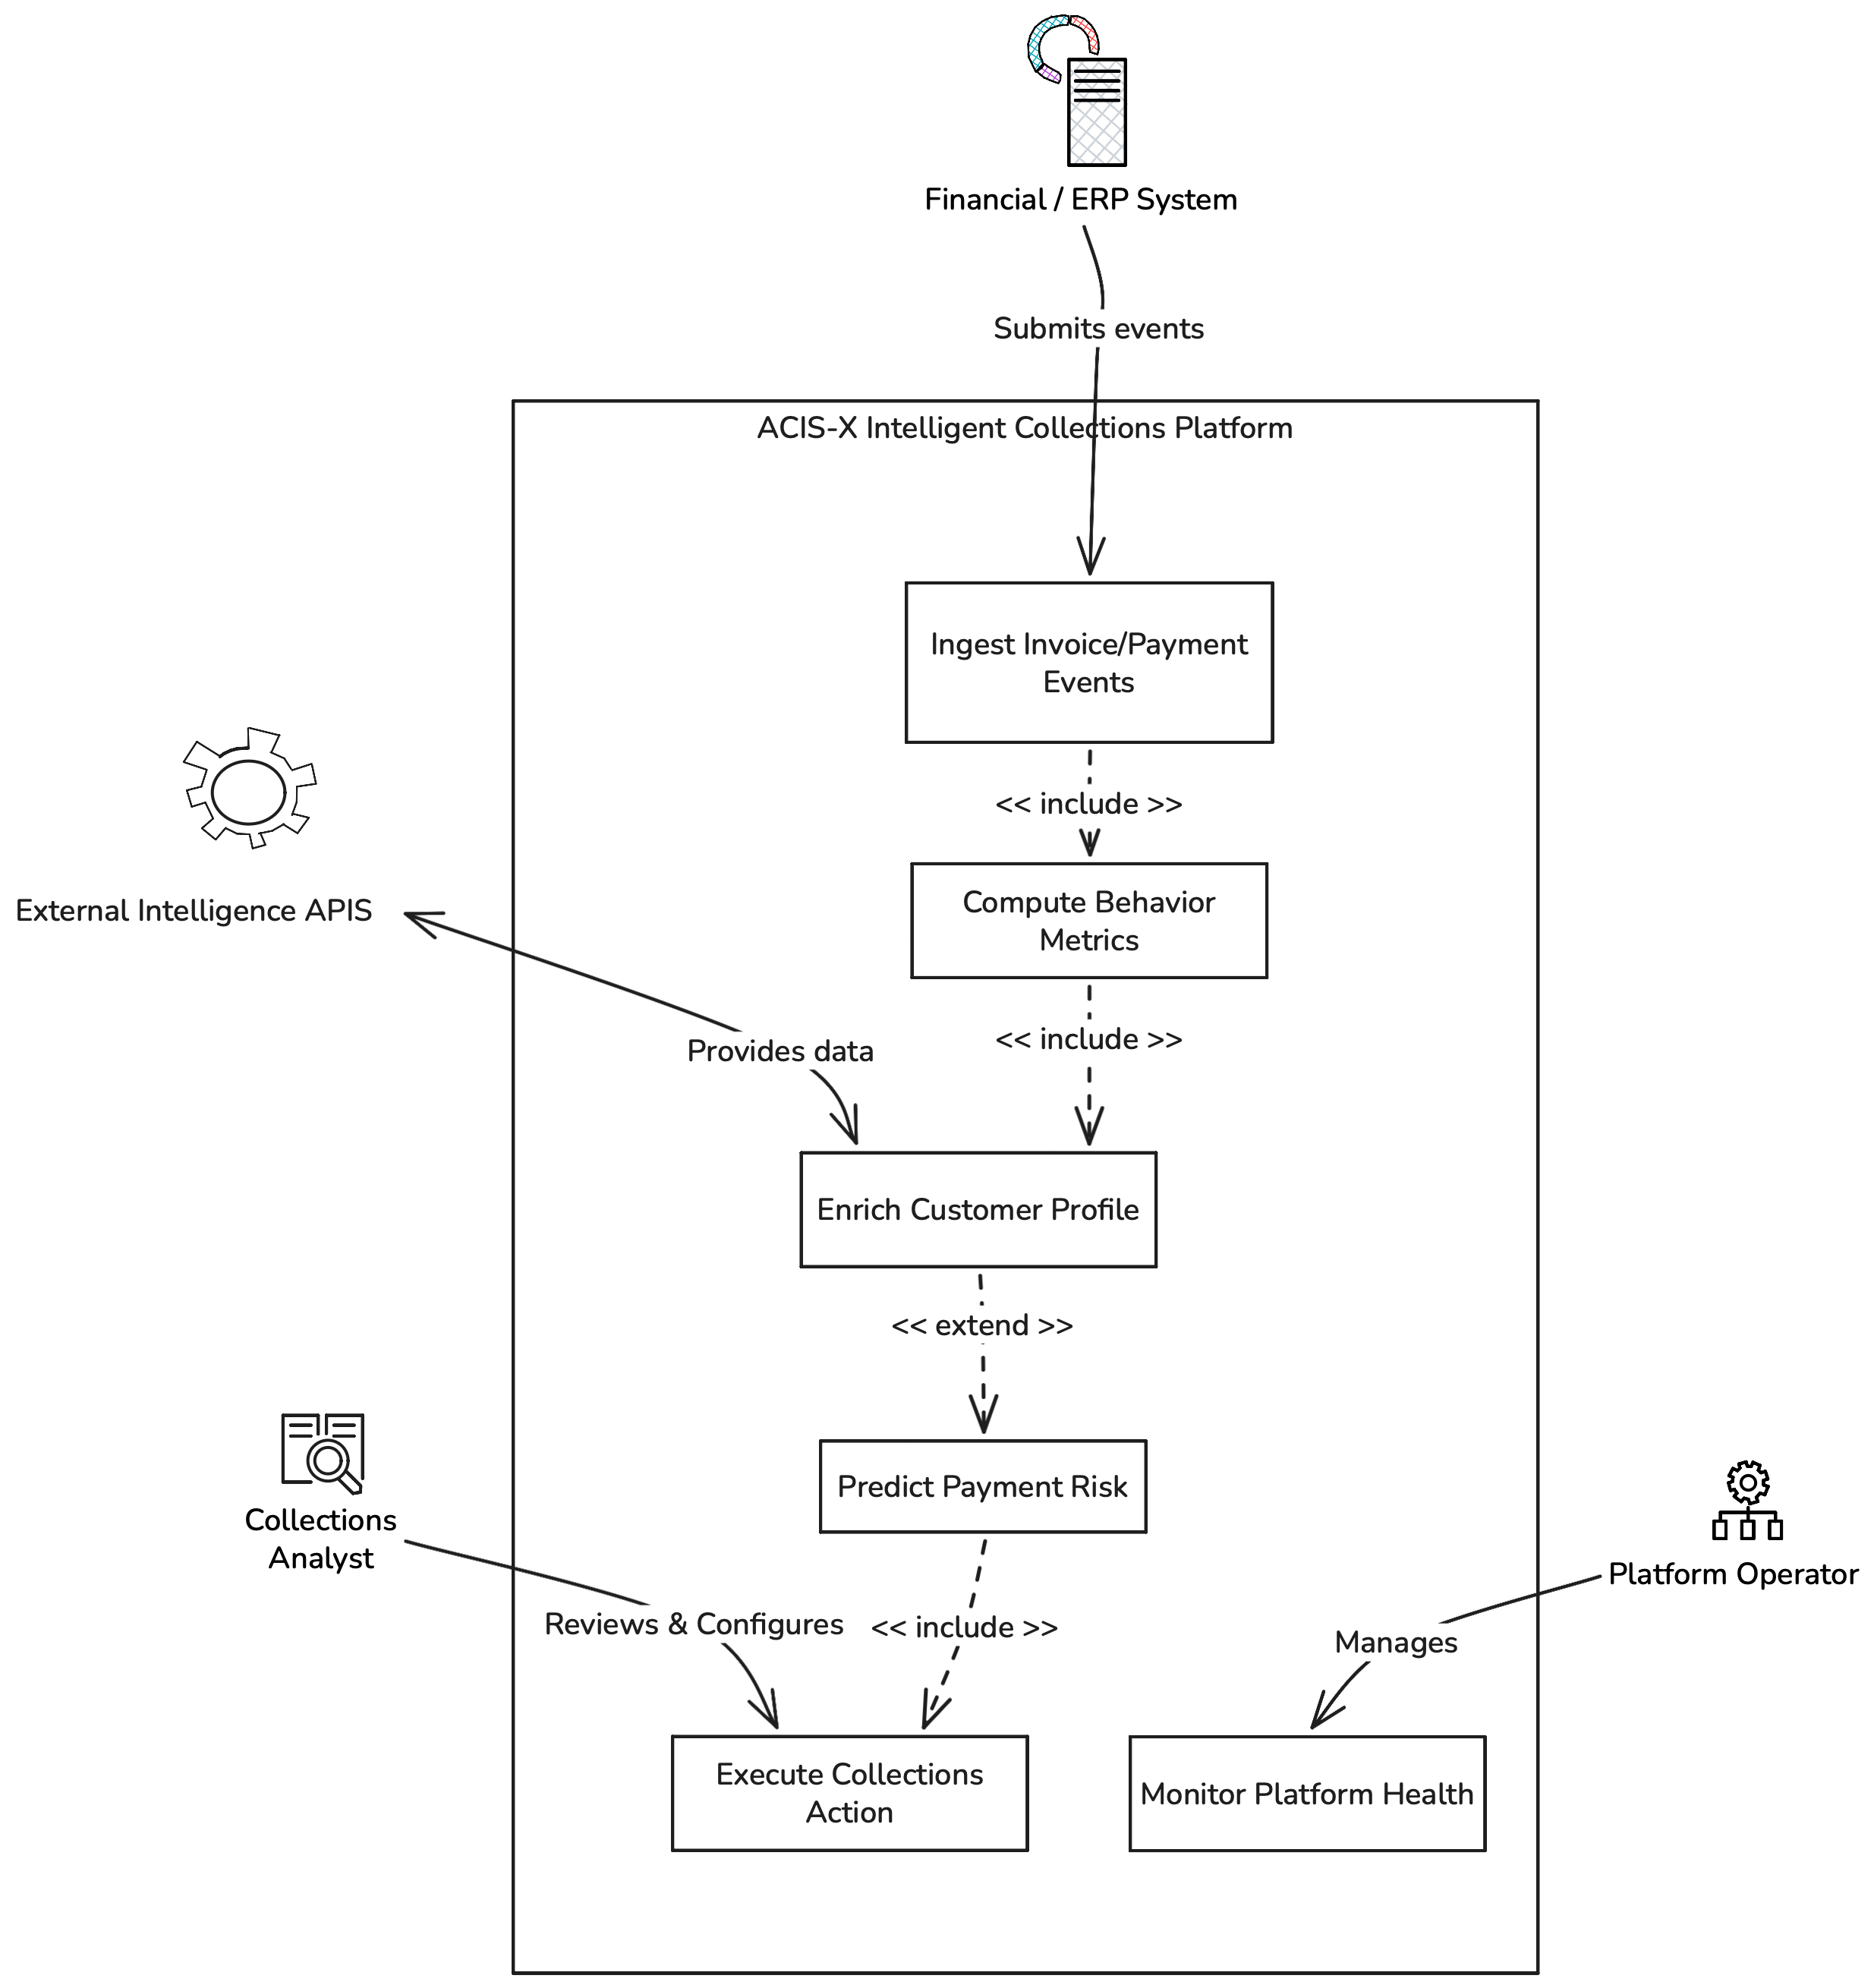
\includegraphics[width=0.7\textwidth]{images/use-case-diag.png}
    \caption{Use case diagram for ACIS-X}
    \label{fig:use_case}
\end{figure}

\subsection{Sequence Diagram}
The Sequence Diagram visualizes the asynchronous, topic-based communication flowing between dedicated agents (e.g., ScenarioGenerator, ExternalData, RiskScoring) and their centralized exchange via the Kafka Event Bus.

\begin{figure}[H]
    \centering
    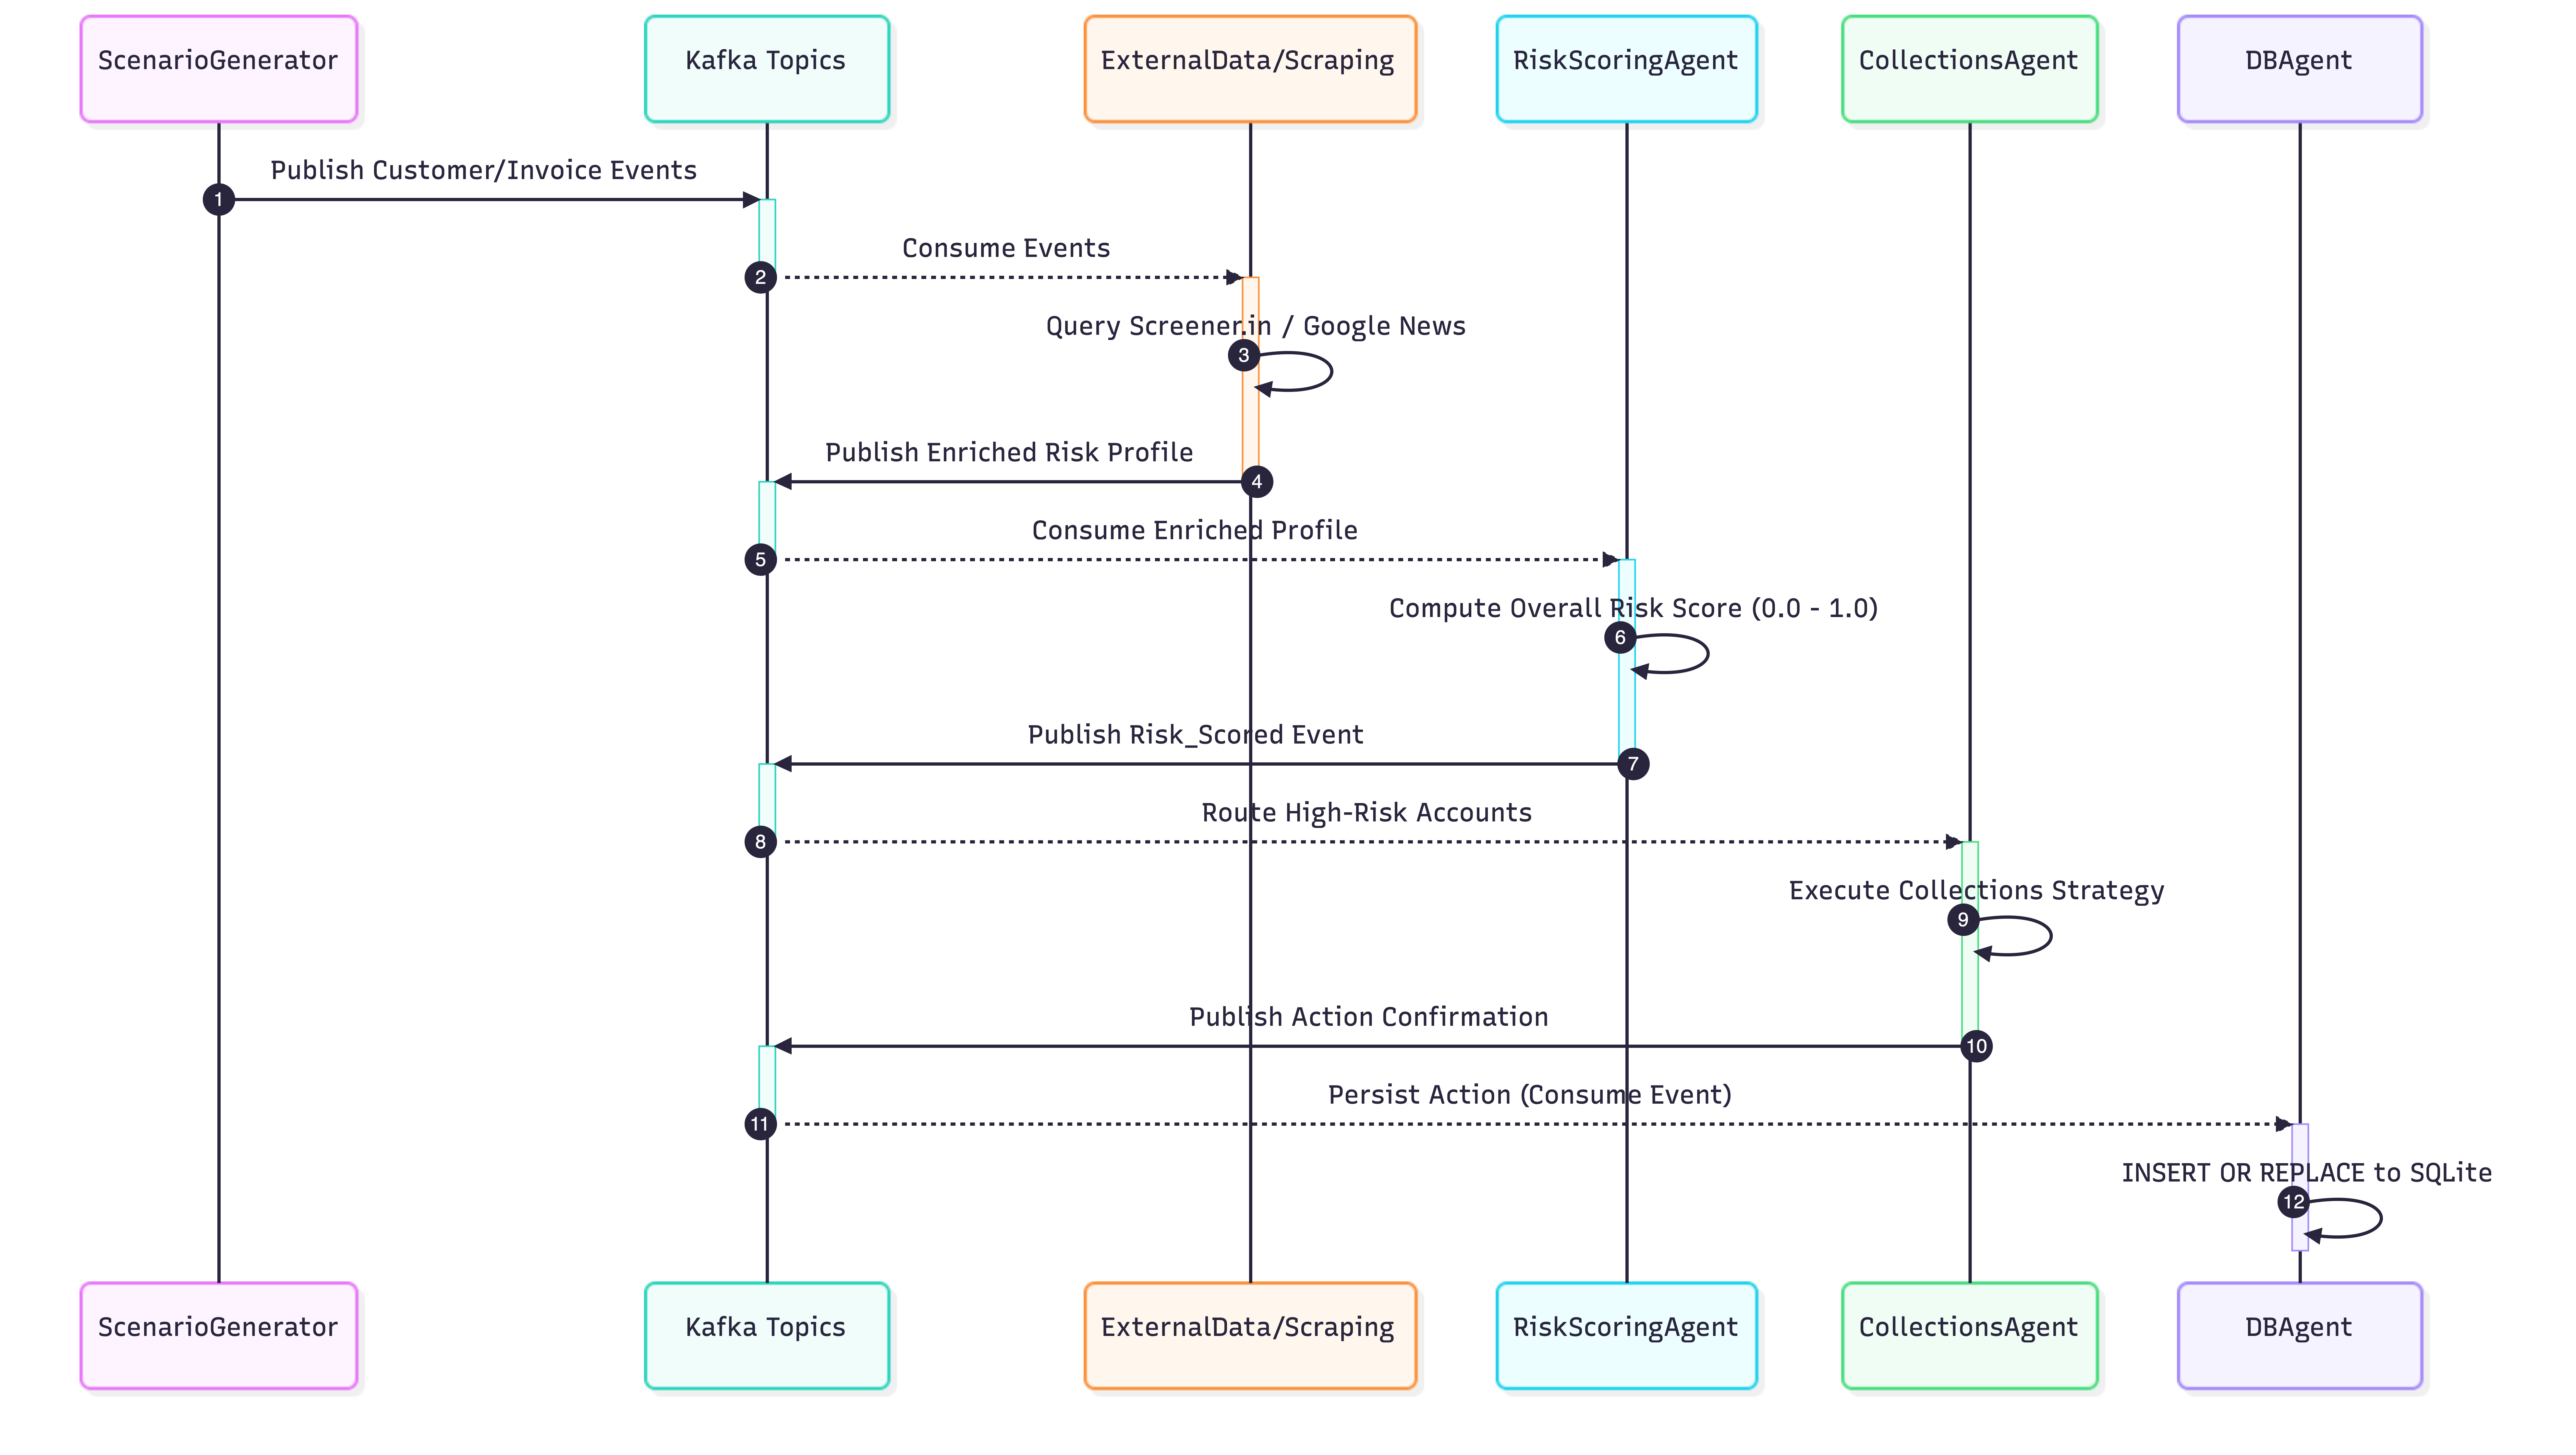
\includegraphics[width=0.9\textwidth]{images/sequence-diag.png}
    \caption{Sequence diagram illustrating event communication flows}
    \label{fig:sequence_diagram}
\end{figure}

\subsection{Activity Diagram}
The Activity Diagram details the step-by-step workflow for the data processing pipeline starting from raw invoice ingestion, progressing to metrics computation and enrichment, and culminating in collections escalations.

\begin{figure}[H]
    \centering
    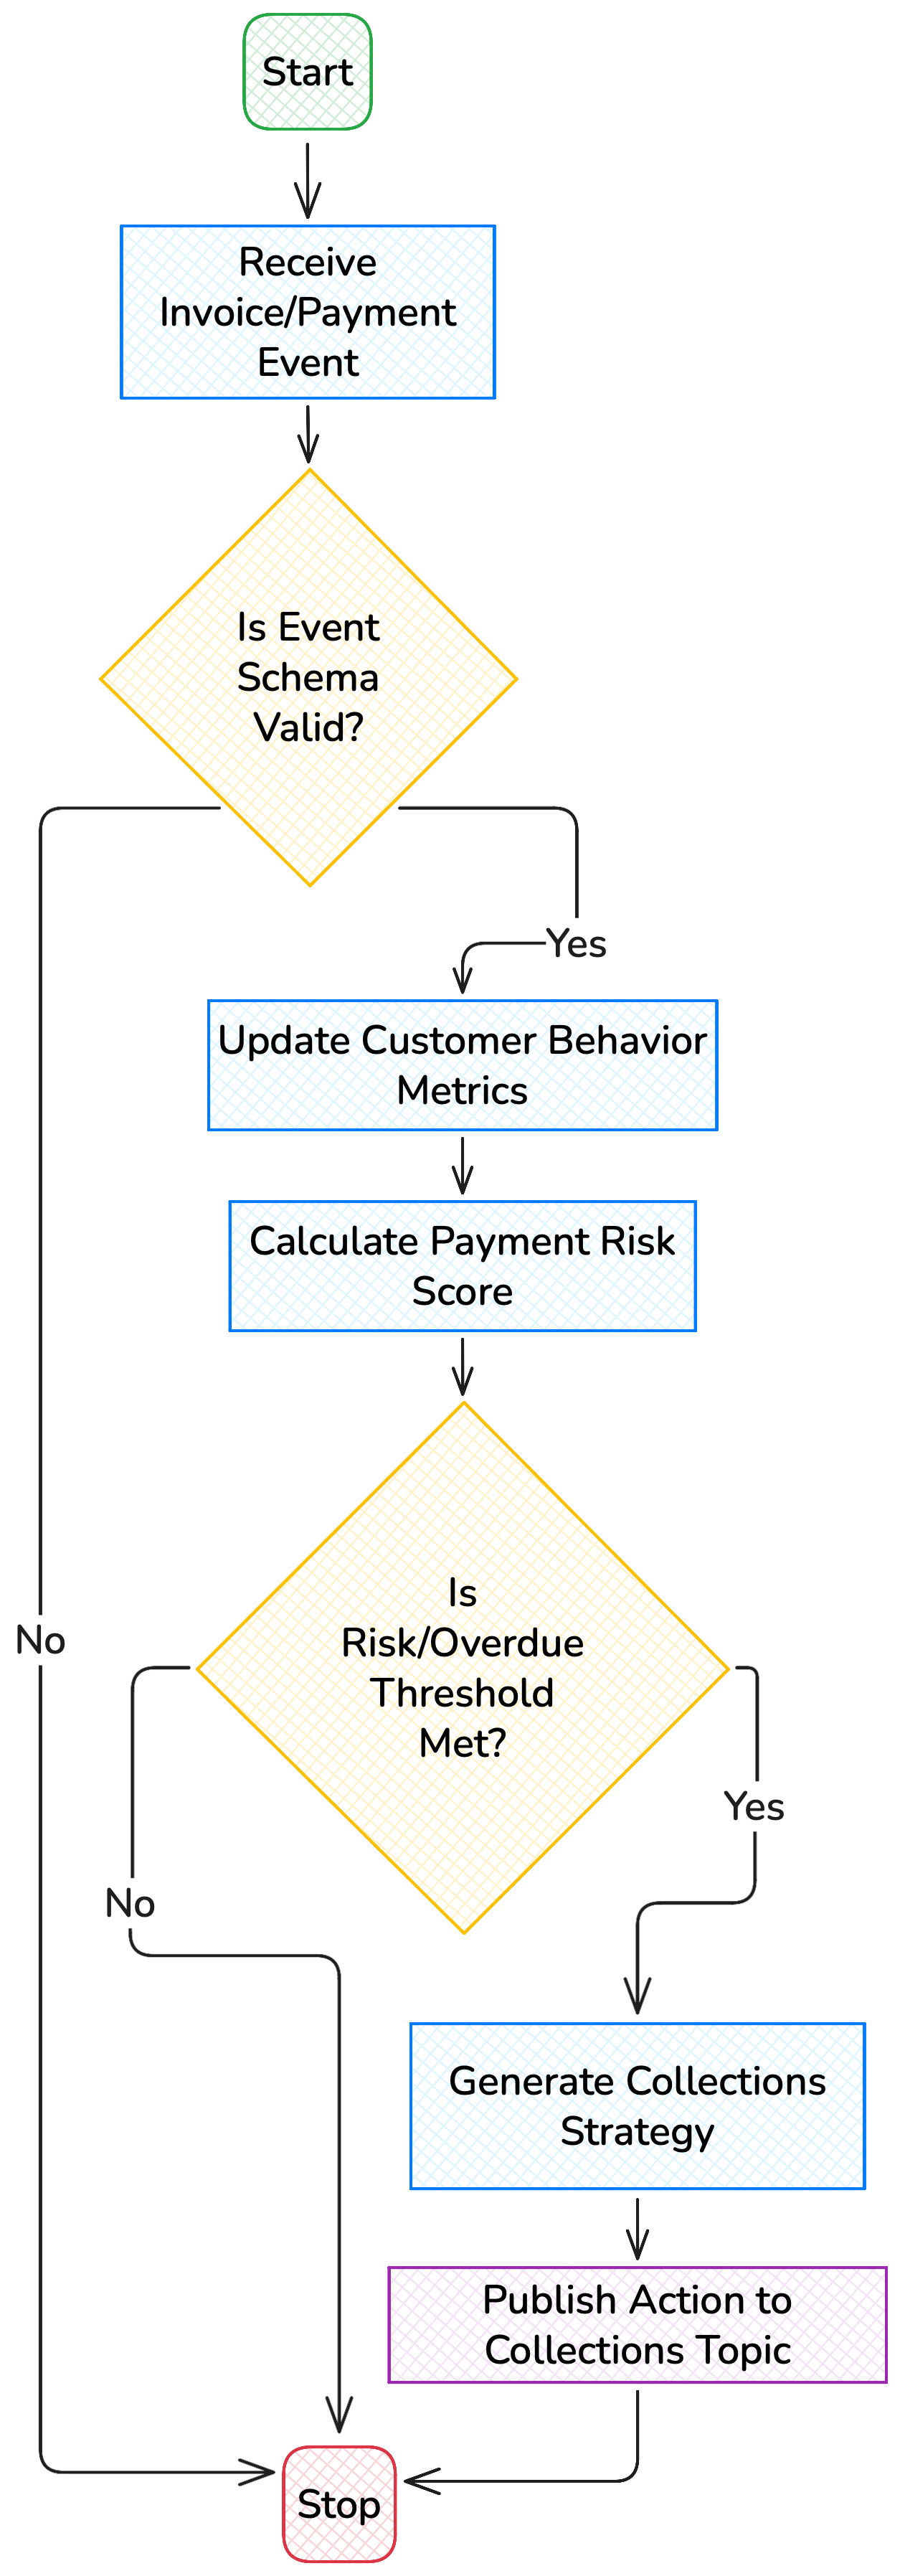
\includegraphics[width=0.45\textwidth]{images/activity-diag.png}
    \caption{Activity diagram mapping out the decision pipeline}
    \label{fig:activity_diagram}
\end{figure}

\subsection{State Chart Diagram}
The State Chart Diagram maps the lifecycle of an account's state within ACIS-X, transitioning between normal operations, an early warning status during overdue detection, and a high-risk state triggering immediate policy/collections interventions.

\begin{figure}[H]
    \centering
    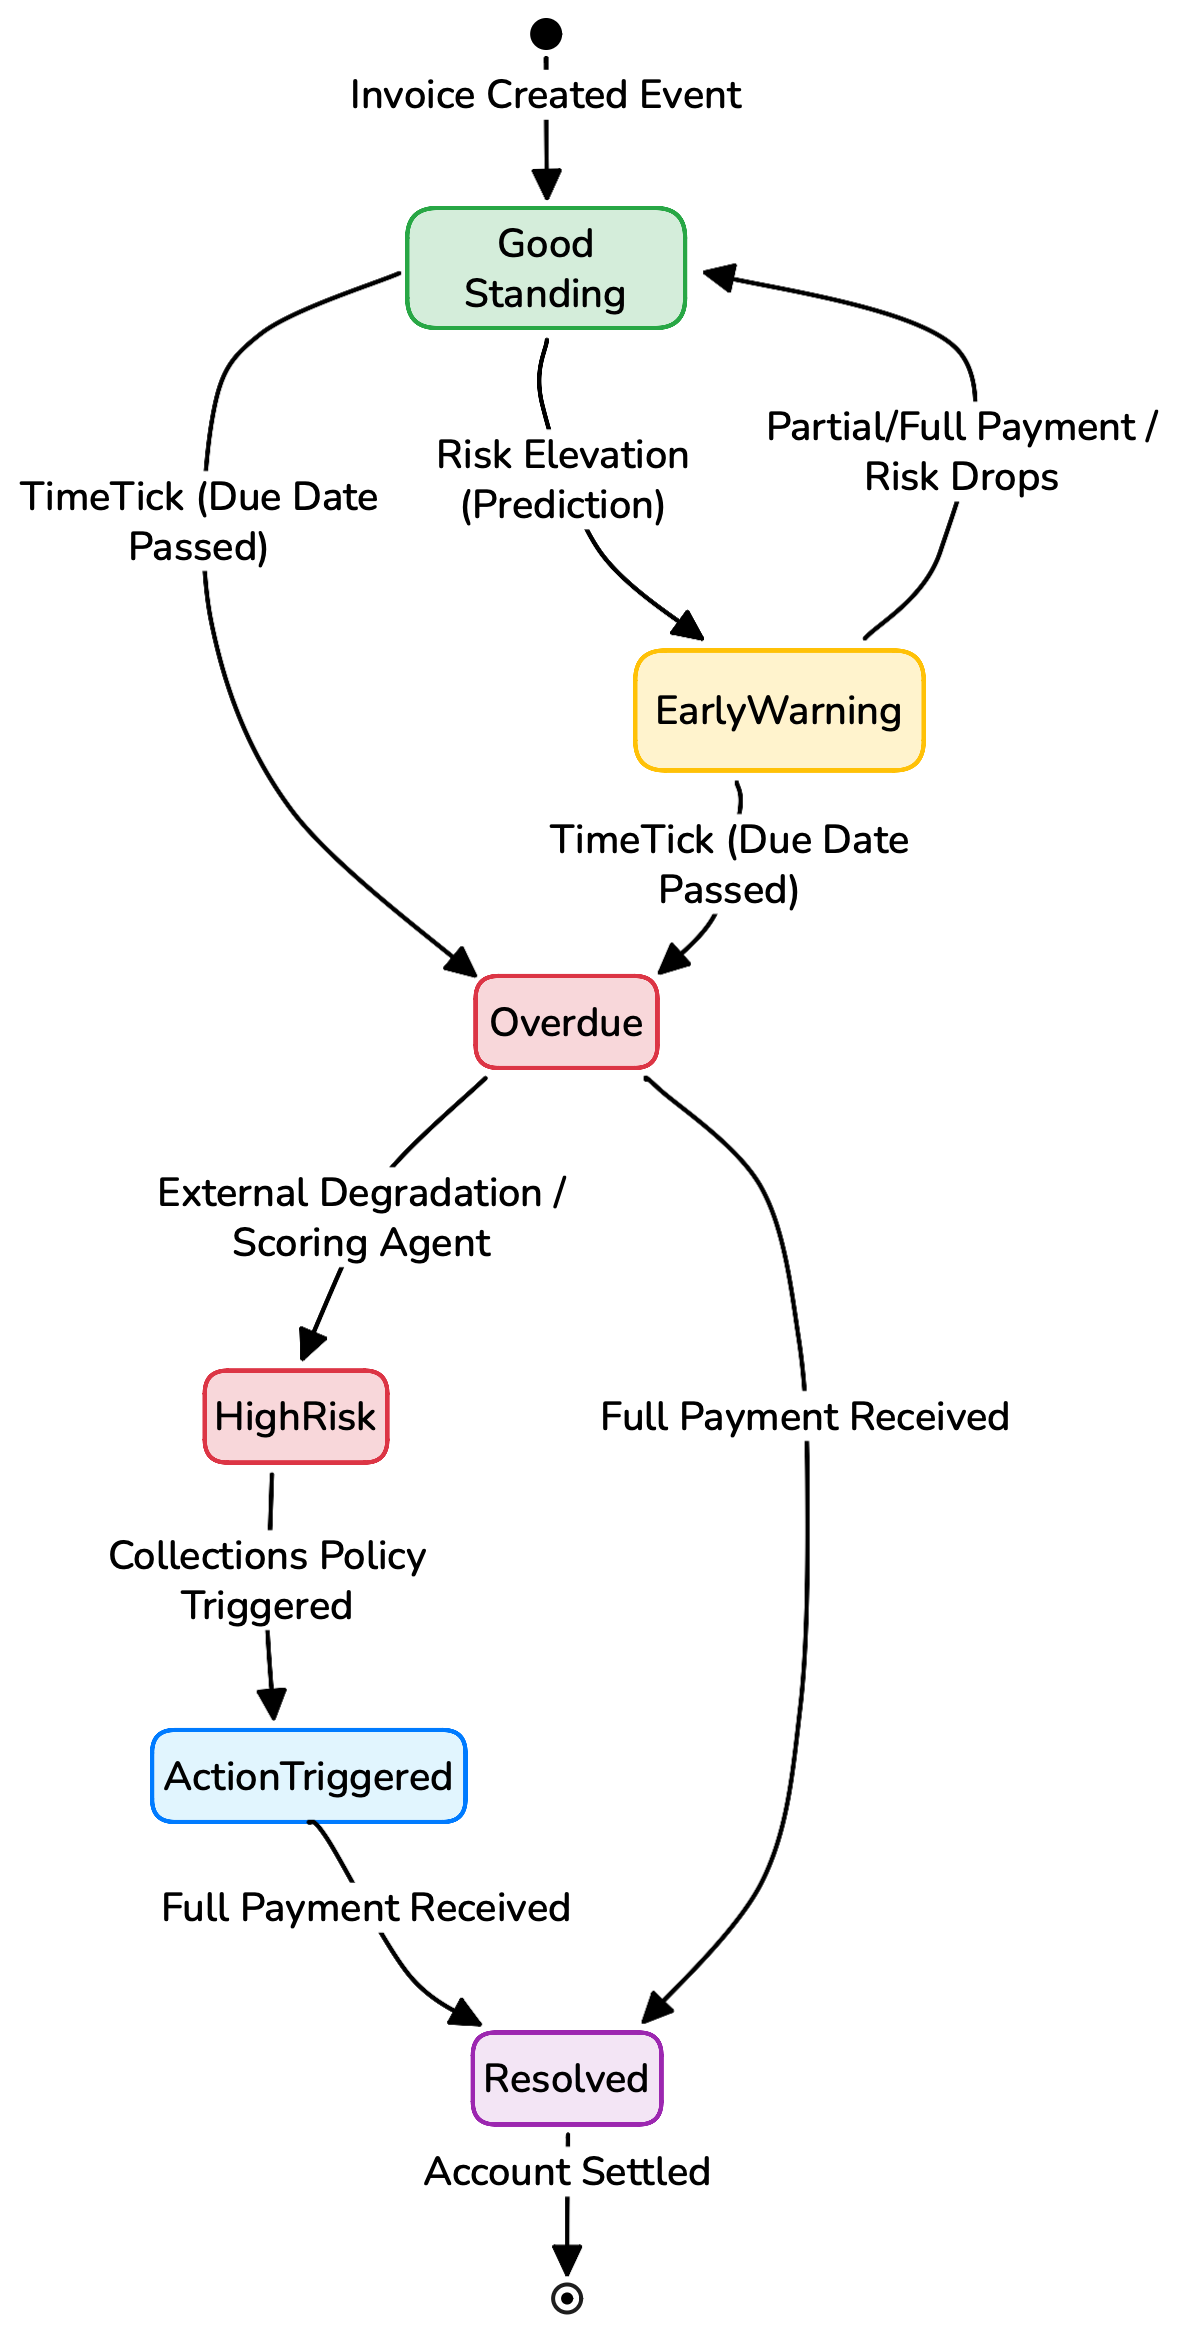
\includegraphics[width=0.55\textwidth]{images/state-chart-diag.png}
    \caption{State chart diagram specifying account state transitions}
    \label{fig:state_chart}
\end{figure}

\section{Software Requirement Specification}
The Software Requirement Specification (SRS) defines what ACIS-X must do and how well it must do it under realistic operational conditions. Requirements are grouped into functional, non-functional, interface/data, and governance-oriented validation requirements.

\subsection{Functional Requirements}
\begin{enumerate}[label=\textbf{\roman*.}]
    \item \textbf{Event Ingestion:} The system must be able to continuously consume customer, invoice, and payment events from Kafka topics.
    \item \textbf{State Computation:} The system must compute and maintain real-time customer behavior metrics and exposure aggregations.
    \item \textbf{External Enrichment:} The system should fetch and integrate external financial and litigation data to enrich customer profiles.
    \item \textbf{Risk Prediction:} It must generate structured invoice-level payment-risk predictions based on unified account data.
    \item \textbf{Action Routing:} The system must evaluate risk scores against policies and trigger appropriate collections actions automatically.
\end{enumerate}

\subsection{Non-Functional Requirements}
\begin{enumerate}[label=\textbf{\roman*.}]
    \item \textbf{Performance:} The platform should process events efficiently with high throughput and minimal latency.
    \item \textbf{Reliability:} The system must ensure continuous operation with automated retry and dead-letter queue (DLQ) mechanisms for fault tolerance.
    \item \textbf{Scalability:} The architecture should scale horizontally by allowing multiple agent replicas within canonical consumer groups.
    \item \textbf{Maintainability:} The modular multi-agent structure and explicit event contracts must support easy updates and independent component lifecycle management.
    \item \textbf{Observability:} The system should emit continuous logs, heartbeats, and metrics to ensure clear diagnostic visibility.
\end{enumerate}

The functional and non-functional requirements above define the SRS baseline for ACIS-X in the same subsection structure used in the reference report.

\chapter{PROJECT PLANNING}

\section{Project Planning}

Project planning is a critical phase for ACIS-X because the system combines event-driven engineering, risk intelligence, operational controls, and reporting workflows. To keep development predictable, planning was broken into implementation streams with clear ownership, weekly checkpoints, and validation gates. The project started approximately three weeks ago, and the backend-heavy architecture and data pipeline components are already underway, while frontend/dashboard work remains pending.

\begin{enumerate}[itemsep=-4pt, label=\textbf{\roman*.}]
    \item \textbf{Requirement Consolidation and Scope Freezing: }
    \vspace{-4pt}
    \begin{itemize}[itemsep=-4pt]
        \item Mapped requirements from architecture docs, runtime code, tests, and deployment guidelines.
        \item Locked Chapter 3 SRS scope around functional and non-functional requirements aligned with the reference format.
    \end{itemize}

    \item \textbf{Architecture and Module Planning: }
    \vspace{-4pt}
    \begin{itemize}[itemsep=-4pt]
        \item Organized work by layers: ingestion/state, enrichment/prediction, scoring/actioning, and control-plane resilience.
        \item Defined development order to prioritize stable event flow before UX and reporting surfaces.
    \end{itemize}

    \item \textbf{Backend Implementation Track: }
    \vspace{-4pt}
    \begin{itemize}[itemsep=-4pt]
        \item Prioritized agent orchestration, topic contracts, persistence paths, and runtime startup/shutdown reliability.
        \item Focused first three weeks on core ACIS-X pipeline correctness and integration readiness.
    \end{itemize}

    \item \textbf{Data and External Integration Track: }
    \vspace{-4pt}
    \begin{itemize}[itemsep=-4pt]
        \item Planned integration of external financial and litigation signals with fallback mechanisms.
        \item Added checkpoints for API timeout behavior, retry strategy, and enrichment consistency.
    \end{itemize}

    \item \textbf{Testing and Validation Track: }
    \vspace{-4pt}
    \begin{itemize}[itemsep=-4pt]
        \item Established unit-first validation using pytest markers and architecture-fix regression tests.
        \item Scheduled integration validation after backend stabilization and before frontend coupling.
    \end{itemize}

    \item \textbf{Performance and Reliability Milestones: }
    \vspace{-4pt}
    \begin{itemize}[itemsep=-4pt]
        \item Planned checkpoints for startup time, lag behavior, memory stability, and consumer-group correctness.
        \item Included self-healing and monitoring verification as mandatory pre-demonstration criteria.
    \end{itemize}

    \item \textbf{Frontend and Visualization Planning: }
    \vspace{-4pt}
    \begin{itemize}[itemsep=-4pt]
        \item Frontend dashboard/workbench was intentionally scheduled after backend API and event contracts matured.
        \item Current status: frontend implementation is pending and is the next major execution block.
    \end{itemize}

    \item \textbf{Documentation and Report Integration: }
    \vspace{-4pt}
    \begin{itemize}[itemsep=-4pt]
        \item Planned chapter-wise documentation in parallel with implementation to reduce end-cycle documentation risk.
        \item Ensured report structure mirrors reference chapter/subheading style while preserving ACIS-X specifics.
    \end{itemize}

    \item \textbf{Risk Management and Mitigation: }
    \vspace{-4pt}
    \begin{itemize}[itemsep=-4pt]
        \item Key risks: external API unreliability, schema drift, event lag spikes, and timeline compression for frontend completion.
        \item Mitigation: fallback data paths, strict event contracts, continuous testing, and phased frontend rollout.
    \end{itemize}

    \item \textbf{Milestone Tracking and Delivery Governance: }
    \vspace{-4pt}
    \begin{itemize}[itemsep=-4pt]
        \item Weekly milestone tracking with completed/in-progress/pending status tags.
        \item Delivery sequencing follows: backend hardening -> frontend completion -> end-to-end validation -> final submission.
    \end{itemize}
\end{enumerate}

\subsection{Scheduling}
Scheduling for ACIS-X is based on an 8-week execution window, with approximately the first 3 weeks already completed. The schedule emphasizes backend-first completion, then frontend implementation, integration, and final validation/documentation.

The schedule in Table~\ref{tab:acis_project_schedule} outlines the planned timeline and current progress state.

\vspace{-4pt}
\begin{longtable}{|L{0.12\textwidth}|L{0.16\textwidth}|L{0.50\textwidth}|L{0.14\textwidth}|}
    \caption{ACIS-X Project Schedule (8-Week Plan)}\label{tab:acis_project_schedule} \\

    \hline
    \textbf{Phase} & \textbf{Week} & \textbf{Task} & \textbf{Status} \\
    \hline
    \endfirsthead

    \multicolumn{4}{c}%
    {\tablename\ \thetable\: \textit{Continued from previous page}} \\
    \hline
    \textbf{Phase} & \textbf{Week} & \textbf{Task} & \textbf{Status} \\
    \hline
    \endhead

    \hline \multicolumn{4}{r}{\textit{Continued on next page}} \\
    \endfoot

    \hline
    \endlastfoot

    Phase 1 & Week 1 & Literature alignment, architecture review, scope definition, environment setup. & Completed \\
    \hline
    Phase 1 & Week 2 & Requirement engineering draft, chapter structuring, runtime/dependency mapping. & Completed \\
    \hline
    Phase 1 & Week 3 & Core backend pipeline refinement, table/LaTeX stabilization, chapter updates. & Completed \\
    \hline
    Phase 2 & Week 4 & Frontend planning finalization, UI wireframe selection, API binding contracts. & Completed \\
    \hline
    Phase 2 & Week 5 & Frontend implementation (dashboards, risk/action views, status panels). & In Progress \\
    \hline
    Phase 3 & Week 6 & End-to-end integration: frontend with event and persistence outputs. & In Progress \\
    \hline
    Phase 3 & Week 7 & System validation, performance checks, bug fixes, UX improvements. & Pending \\
    \hline
    Phase 4 & Week 8 & Final report polishing, consolidated testing evidence, final submission prep. & Pending \\
\end{longtable}

\chapter{SYSTEM DESIGN}

\section{System Architecture}
The system architecture of ACIS-X is designed as an event-driven, multi-agent platform for intelligent accounts receivable monitoring and collections decision support. The architecture separates data ingestion, customer-state construction, external enrichment, prediction, risk scoring, collections actioning, persistence, and runtime supervision into independent but coordinated modules.

At the center of the architecture is a Kafka-based event backbone. Each major business event, such as customer creation, invoice generation, payment posting, metric computation, risk scoring, and collections action, is published to a dedicated topic. This allows agents to operate independently while still participating in a unified processing workflow. The event-based design also improves traceability because each decision can be connected back to the events and derived signals that produced it.

\begin{figure}[H]
    \centering
    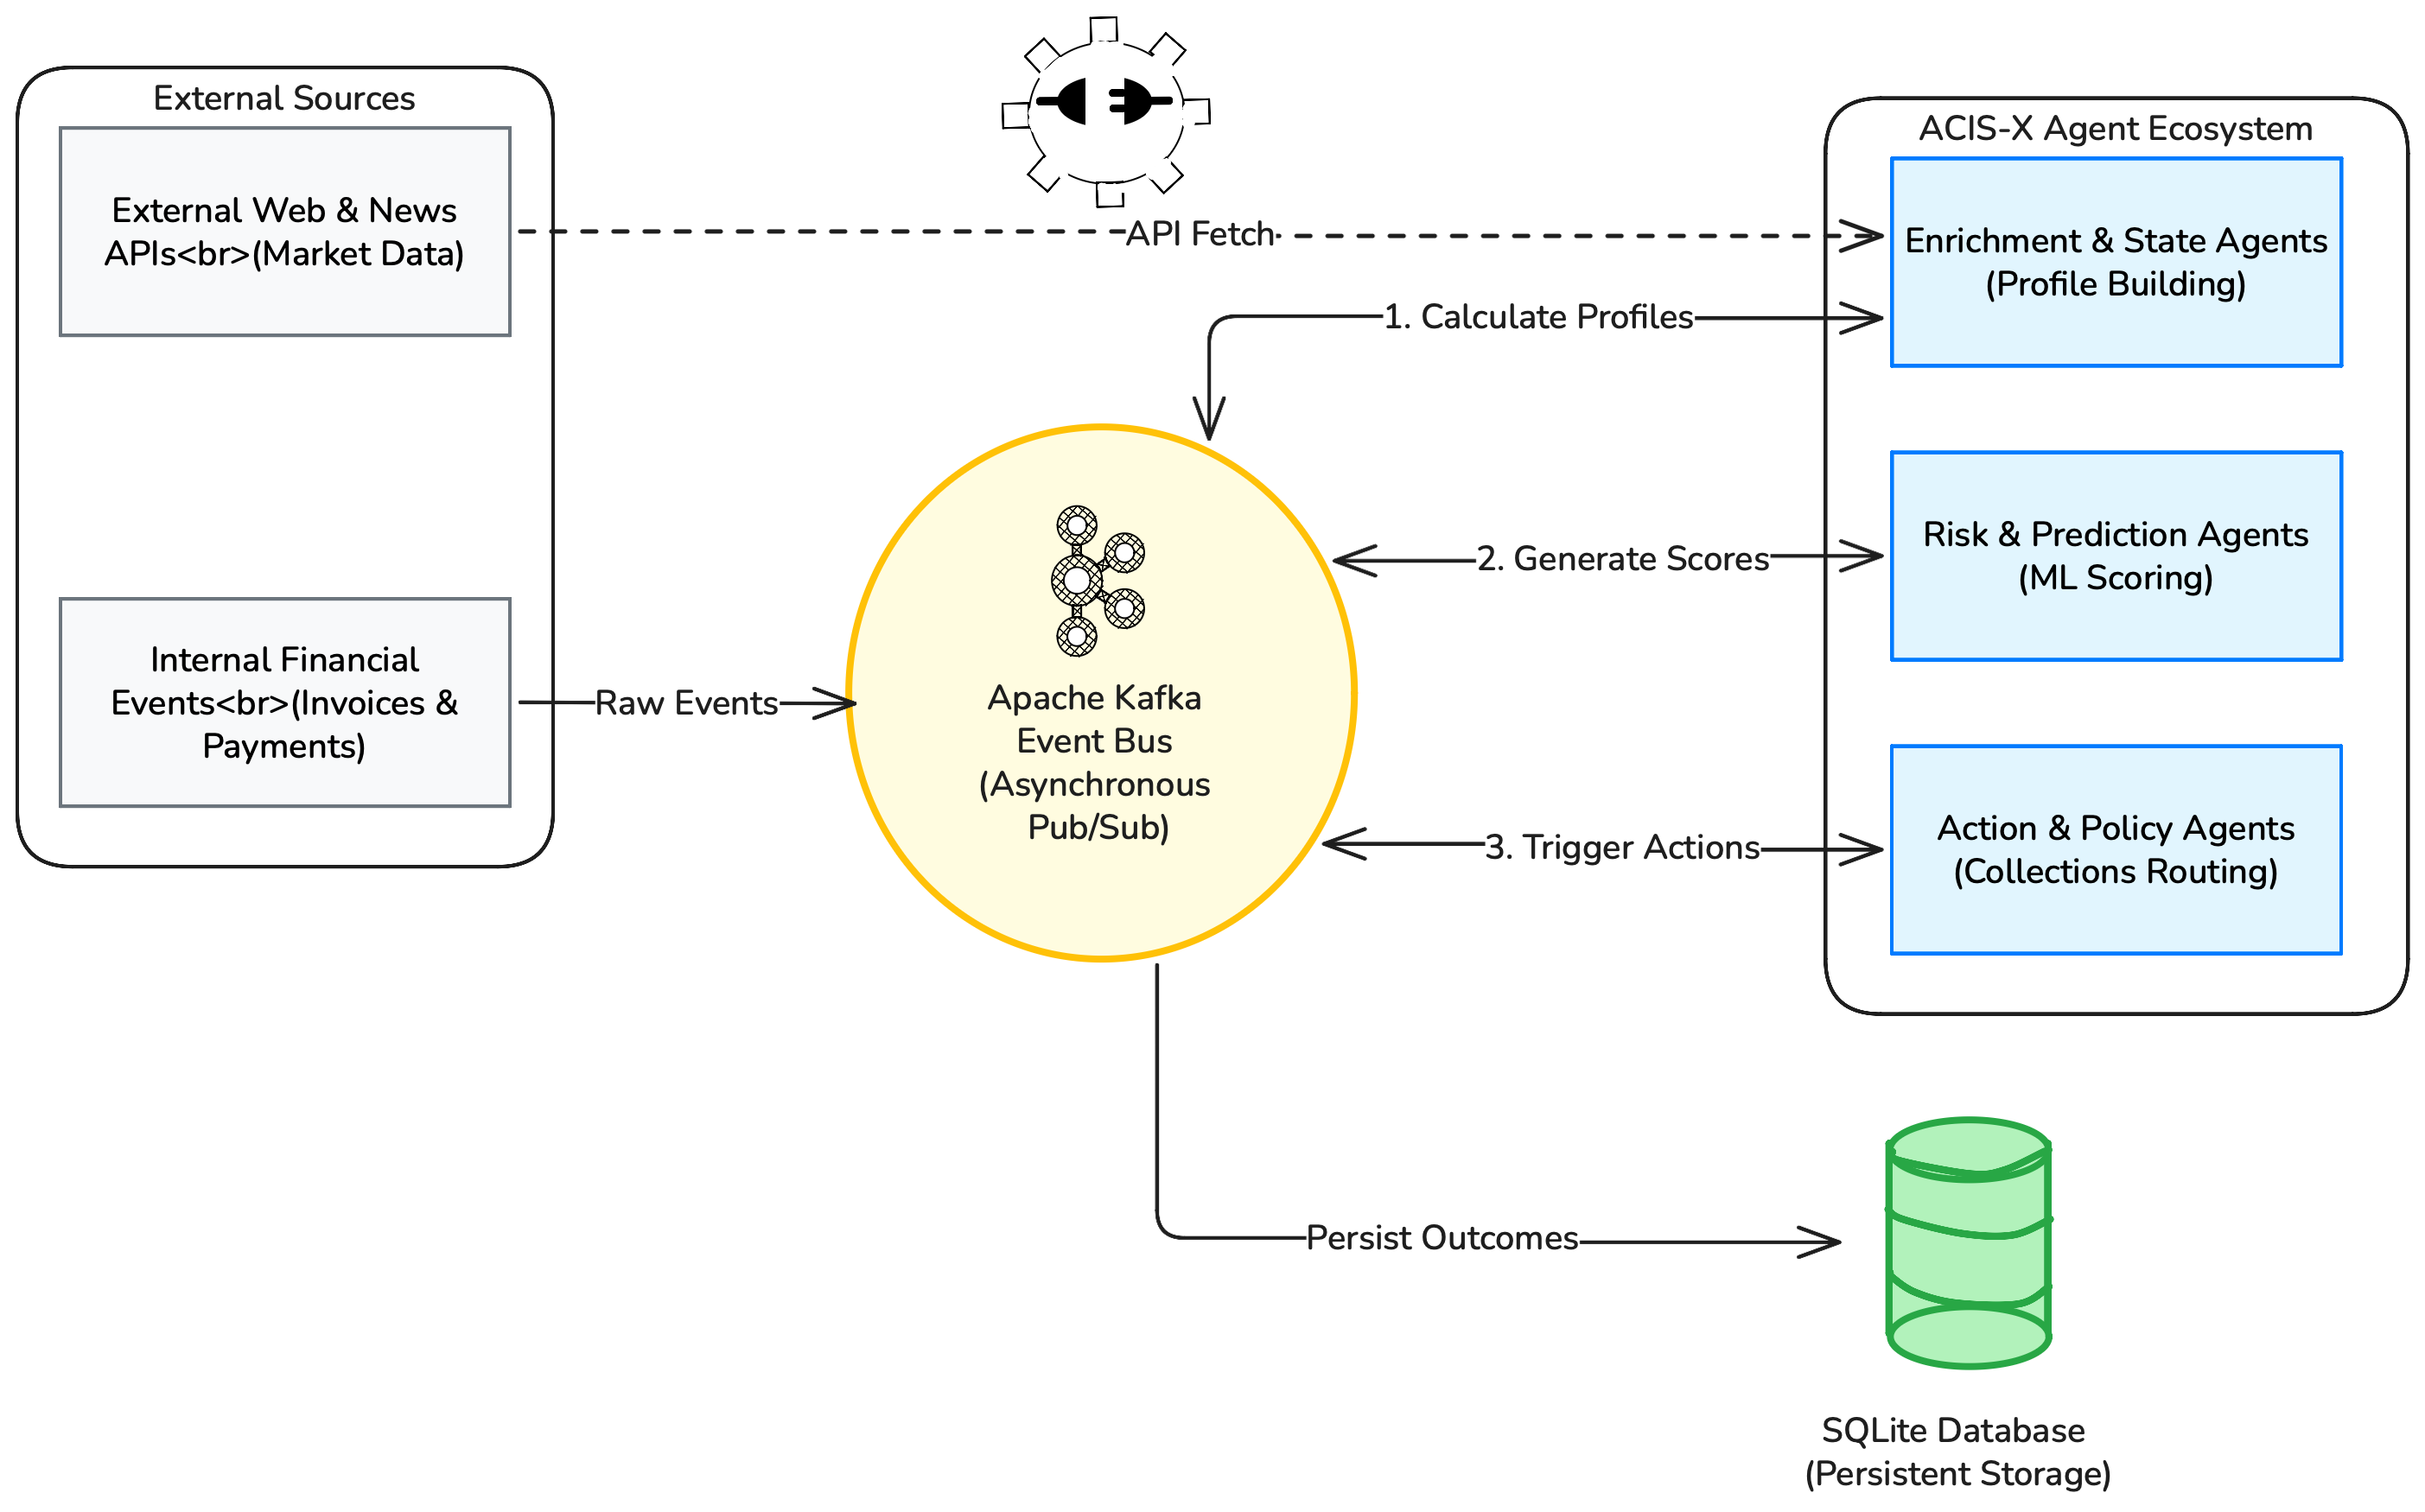
\includegraphics[width=0.9\textwidth]{images/architecture-diag.png}
    \caption{System architecture of ACIS-X}
    \label{fig:system_architecture}
\end{figure}

As shown in Fig~\ref{fig:system_architecture}, ACIS-X consists of five major architectural layers. The input layer provides customer, invoice, payment, and external source information. The event bus layer routes this information through Kafka topics. The agent layer performs state computation, enrichment, aggregation, prediction, risk scoring, and collections actioning. The storage and query layer persists events and derived records using SQLite, while QueryAgent and MemoryAgent provide structured access to state. The user and operations layer exposes the processed outputs through the FastAPI backend-for-frontend, React dashboard, monitoring services, registry services, and self-healing runtime modules.

The architecture is intentionally modular. Business agents focus on receivables intelligence, while runtime agents focus on operational reliability. This separation ensures that failures in monitoring, recovery, or placement logic do not directly alter the business decision rules, and business logic can evolve without rewriting the runtime orchestration layer.

\section{Component Design / Module Decomposition}
The component design of ACIS-X decomposes the platform into specialized agents and services. Each component has a clearly defined responsibility, communicates using event contracts, and produces outputs that can be consumed by downstream modules. This design supports maintainability, testing, and future extension of the platform.

\begin{figure}[H]
    \centering
    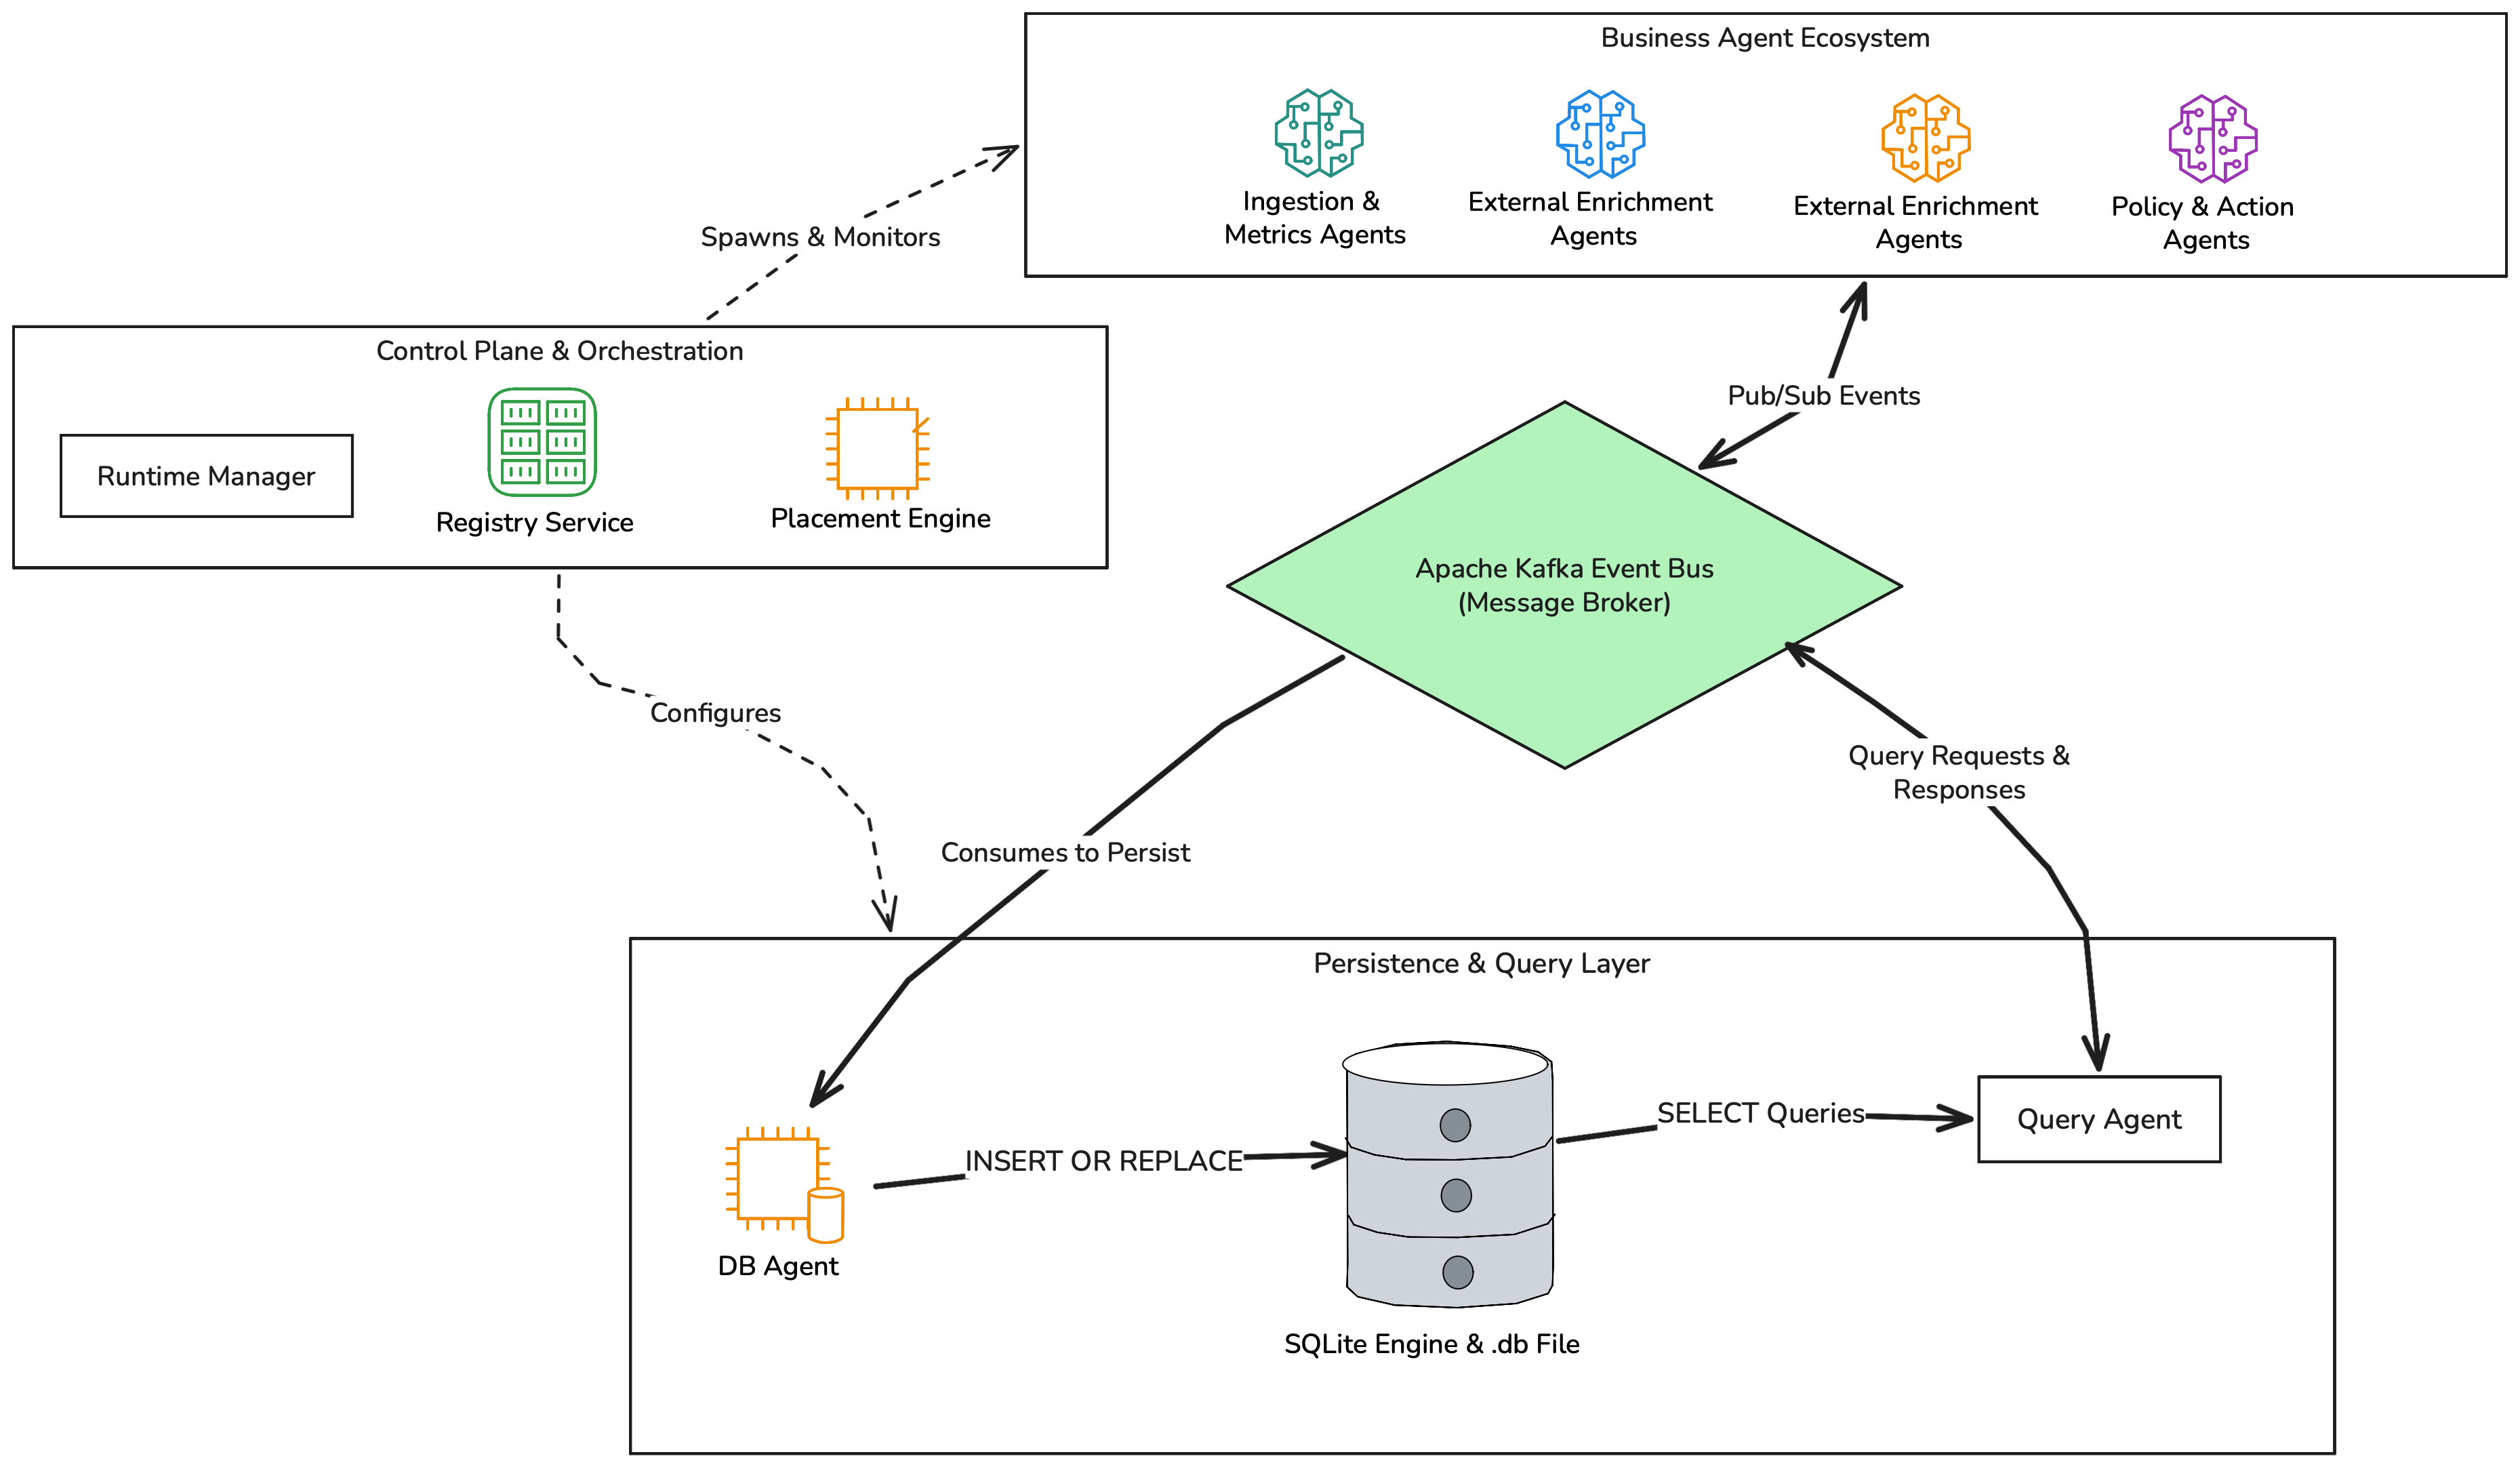
\includegraphics[width=0.9\textwidth]{images/components-diag.png}
    \caption{Component design of ACIS-X}
    \label{fig:component_design}
\end{figure}

Fig~\ref{fig:component_design} shows the main functional modules of the system. ScenarioGeneratorAgent produces simulated operational events. CustomerStateAgent converts invoice and payment behavior into customer metrics. ExternalDataAgent and ExternalScrapingAgent enrich customer context with external signals. AggregatorAgent combines internal and external evidence into a broader customer profile. PaymentPredictionAgent estimates payment risk for open invoices, and RiskScoringAgent converts prediction and context into final risk decisions. CollectionsAgent uses those decisions to recommend appropriate collections actions.

The persistence and query components support the business agents. DBAgent stores events, customer records, invoices, payments, metrics, risk profiles, and collections actions. QueryAgent responds to structured read requests, while MemoryAgent maintains fast runtime context for frequently used customer state. Operational components such as RegistryService, RuntimeManager, MonitoringAgent, PlacementEngine, SelfHealingAgent, and DLQMonitorAgent supervise agent health, recovery, placement, and failed-event handling.

\vspace{-4pt}
\begin{longtable}{|L{0.23\textwidth}|L{0.33\textwidth}|L{0.20\textwidth}|L{0.16\textwidth}|}
    \caption{Core Components of ACIS-X}\label{tab:acis_components} \\

    \hline
    \textbf{Component} & \textbf{Responsibility} & \textbf{Main Input} & \textbf{Main Output} \\
    \hline
    \endfirsthead

    \multicolumn{4}{c}%
    {\tablename\ \thetable\: \textit{Continued from previous page}} \\
    \hline
    \textbf{Component} & \textbf{Responsibility} & \textbf{Main Input} & \textbf{Main Output} \\
    \hline
    \endhead

    \hline \multicolumn{4}{r}{\textit{Continued on next page}} \\
    \endfoot

    \hline
    \endlastfoot

    ScenarioGeneratorAgent & Generates sample customer, invoice, and payment activity for simulation and validation. & Scenario settings & Customer, invoice, and payment events \\
    \hline
    CustomerStateAgent & Computes customer-level receivables metrics from invoice and payment behavior. & Invoice and payment events & Customer metrics \\
    \hline
    ExternalDataAgent & Collects structured external financial or company-level enrichment data. & Customer identity & External financial metrics \\
    \hline
    ExternalScrapingAgent & Extracts litigation, news, or web-based risk indicators related to customers. & Customer/company profile & External risk indicators \\
    \hline
    AggregatorAgent & Combines internal metrics and external indicators into a consolidated risk profile. & Metrics and enrichment data & Aggregated risk profile \\
    \hline
    PaymentPredictionAgent & Estimates payment delay or non-payment likelihood for open invoices. & Invoice and customer metrics & Payment prediction \\
    \hline
    RiskScoringAgent & Produces final risk scores and risk bands using prediction and context. & Prediction and profile data & Risk score event \\
    \hline
    CollectionsAgent & Converts risk outcomes into prioritized collections recommendations. & Risk score event & Collections action \\
    \hline
    DBAgent & Persists raw events and derived records into the local database. & Domain and system events & SQLite records \\
    \hline
    QueryAgent & Serves structured read requests for agents and the API layer. & Query requests & Query responses \\
    \hline
    MemoryAgent & Maintains fast runtime customer and decision context. & Domain events & Cached state \\
    \hline
    MonitoringAgent & Tracks runtime health, heartbeats, lag, and error conditions. & Health and system events & Health status \\
    \hline
    SelfHealingAgent & Initiates recovery actions when agents become unhealthy or fail. & Health status & Recovery action \\
    \hline
    RegistryService & Maintains active agent identity, status, and capability metadata. & Agent registration & Agent registry state \\
\end{longtable}

\section{Interface Design}
The interface design of ACIS-X defines how agents, storage, external sources, and the user-facing dashboard communicate with each other. Since the system is event-driven, most internal interfaces are asynchronous Kafka topics. Each topic represents a specific type of event and allows producers and consumers to remain loosely coupled.

\begin{figure}[H]
    \centering
    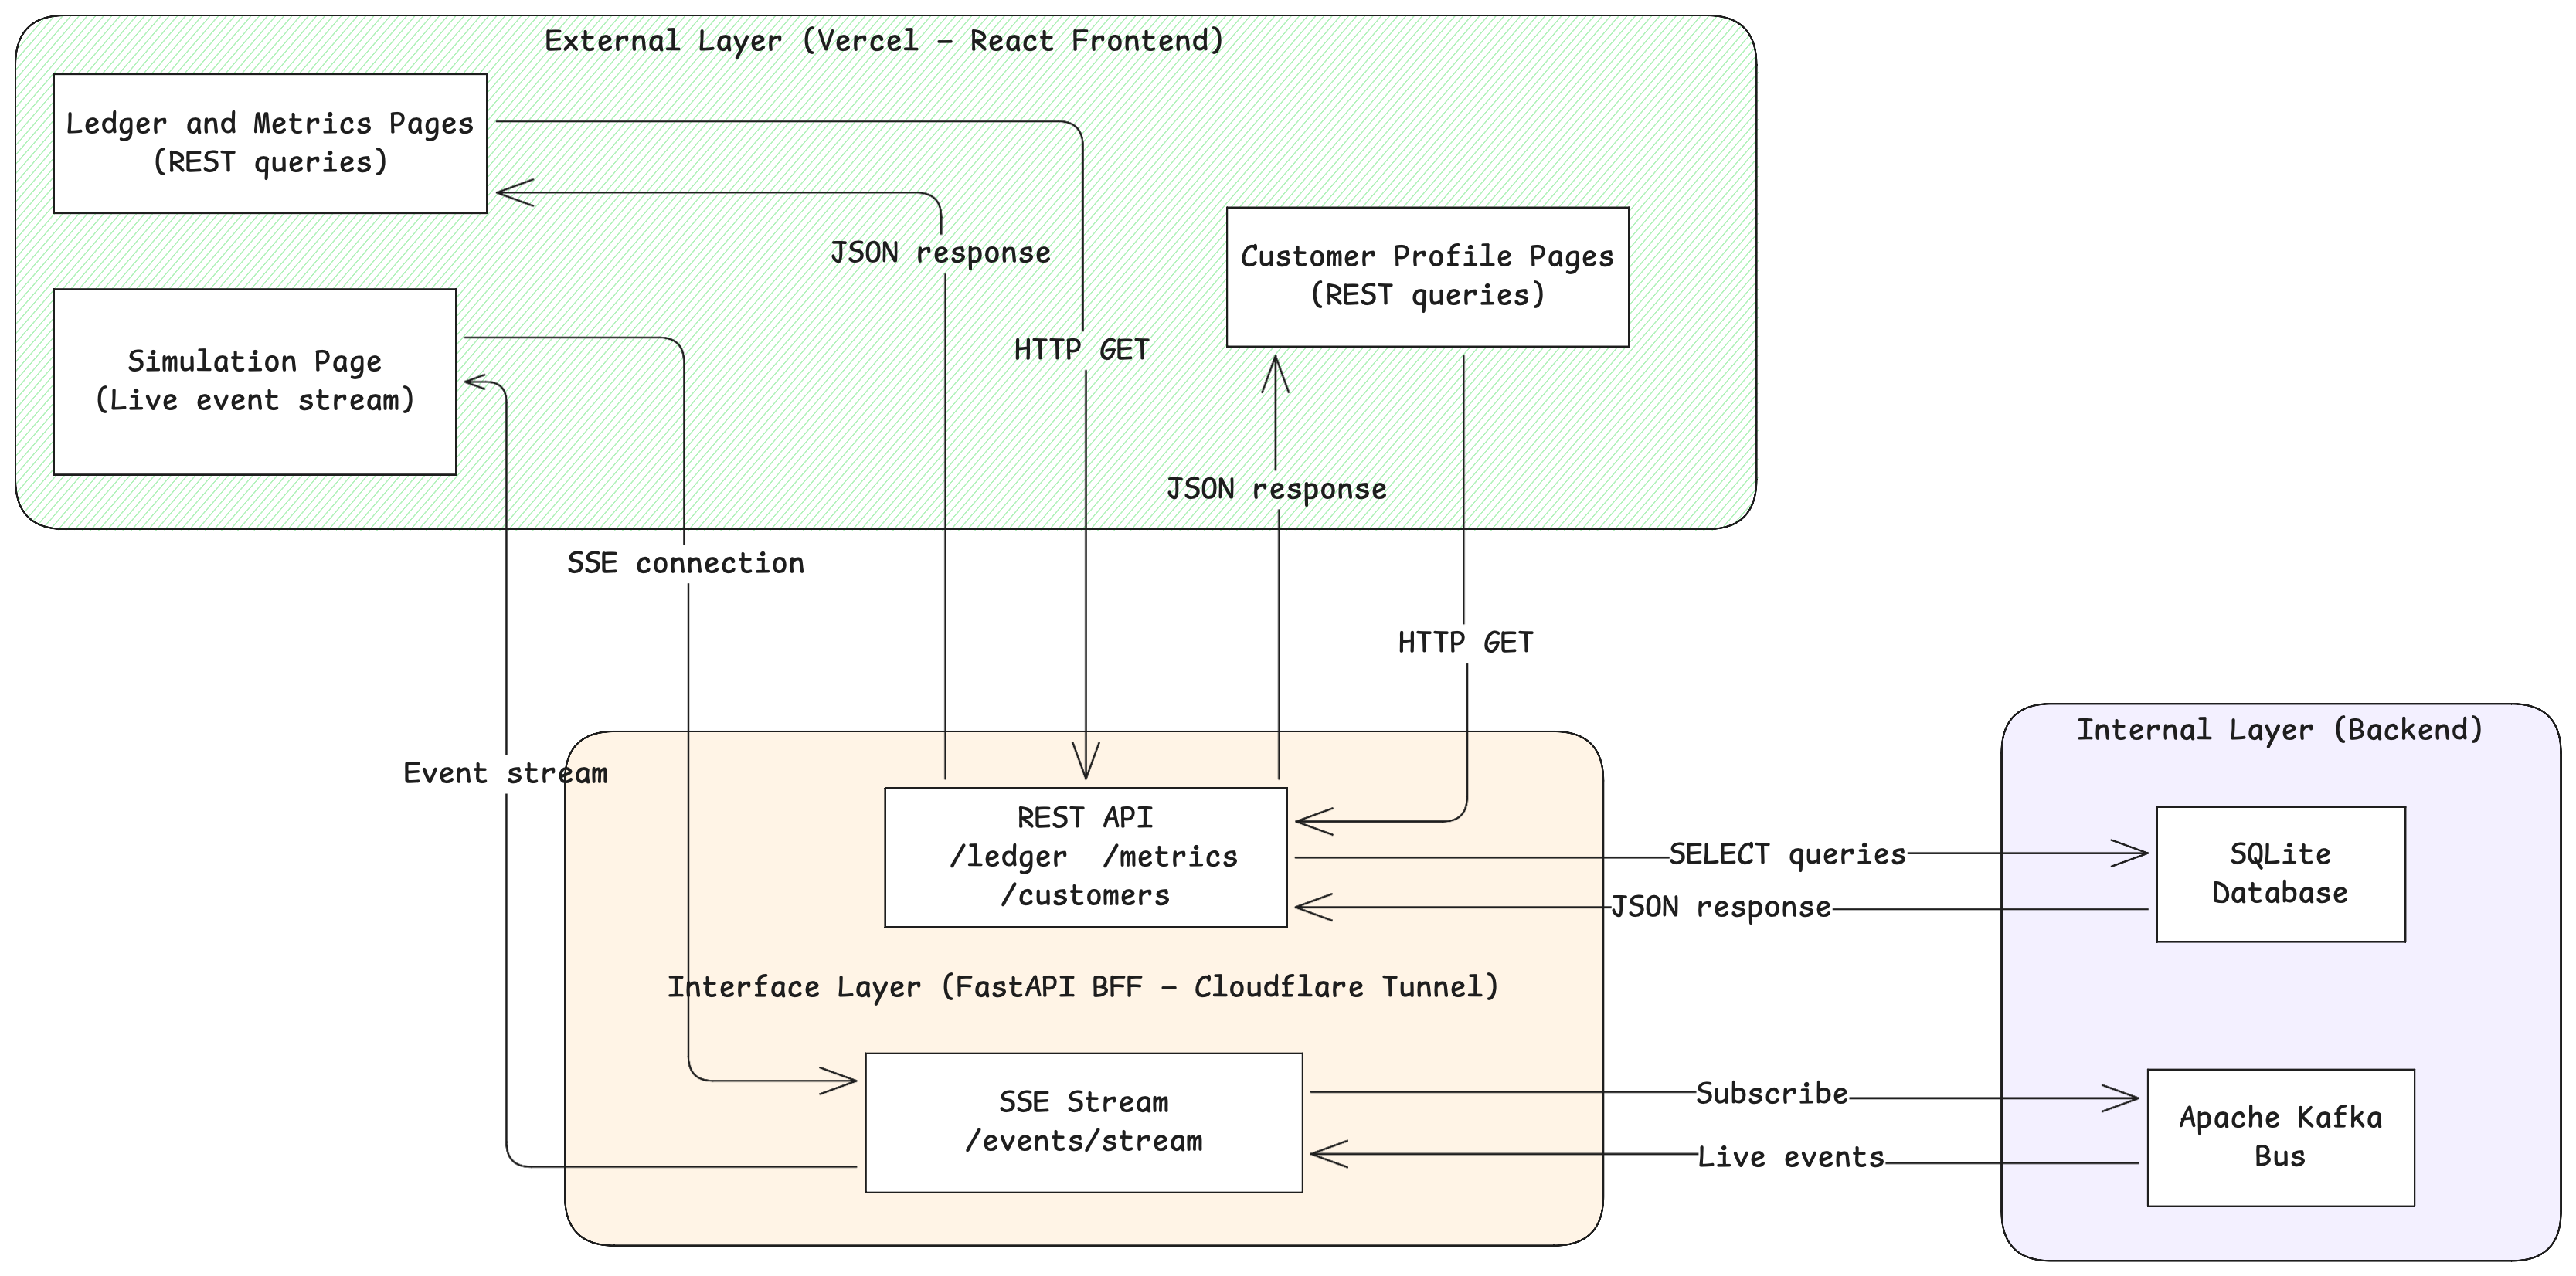
\includegraphics[width=0.9\textwidth]{images/interface-diag.png}
    \caption{Interface design of ACIS-X}
    \label{fig:interface_design}
\end{figure}

As represented in Fig~\ref{fig:interface_design}, ACIS-X uses four primary interface categories. Internal interfaces connect agents through Kafka topics. External interfaces allow enrichment agents to access financial, litigation, news, or company-related data. Persistence interfaces connect DBAgent and QueryAgent with the SQLite database. User-facing interfaces expose risk profiles, collections actions, metrics, and runtime status through the FastAPI backend and React dashboard.

The topic interface is the most important internal communication mechanism. It allows the system to process events incrementally and supports future scaling by adding more producers or consumers without changing the entire architecture.

\vspace{-4pt}
\begin{longtable}{|L{0.22\textwidth}|L{0.23\textwidth}|L{0.25\textwidth}|L{0.22\textwidth}|}
    \caption{Kafka Topic Interface Summary}\label{tab:kafka_topic_interfaces} \\

    \hline
    \textbf{Topic} & \textbf{Producer} & \textbf{Consumer} & \textbf{Purpose} \\
    \hline
    \endfirsthead

    \multicolumn{4}{c}%
    {\tablename\ \thetable\: \textit{Continued from previous page}} \\
    \hline
    \textbf{Topic} & \textbf{Producer} & \textbf{Consumer} & \textbf{Purpose} \\
    \hline
    \endhead

    \hline \multicolumn{4}{r}{\textit{Continued on next page}} \\
    \endfoot

    \hline
    \endlastfoot

    acis.customers & ScenarioGeneratorAgent & DBAgent, MemoryAgent, risk/profile agents & Customer master events \\
    \hline
    acis.invoices & ScenarioGeneratorAgent & DBAgent, CustomerStateAgent, PaymentPredictionAgent & Invoice lifecycle data \\
    \hline
    acis.payments & ScenarioGeneratorAgent & DBAgent, CustomerStateAgent & Payment behavior data \\
    \hline
    acis.metrics & CustomerStateAgent, enrichment agents & AggregatorAgent, PaymentPredictionAgent, DBAgent & Derived customer metrics \\
    \hline
    acis.predictions & PaymentPredictionAgent & RiskScoringAgent, DBAgent & Invoice-level prediction output \\
    \hline
    acis.risk & AggregatorAgent, RiskScoringAgent & CollectionsAgent, DBAgent, dashboard layer & Customer and invoice risk state \\
    \hline
    acis.collections & CollectionsAgent & DBAgent, dashboard layer & Collections recommendation output \\
    \hline
    acis.query.request & API layer or agents & QueryAgent & Structured read request \\
    \hline
    acis.query.response & QueryAgent & API layer or requesting agent & Structured query result \\
    \hline
    acis.agent.health & Runtime agents & MonitoringAgent, SelfHealingAgent & Agent health and heartbeat tracking \\
    \hline
    acis.dlq & Failed processors & DLQMonitorAgent & Failed-event inspection and recovery \\
\end{longtable}

\section{Data Structure Design}
The data structure design of ACIS-X is centered on structured events and persistent domain records. Events are used for communication between agents, while database records are used for durable storage and later query. This separation allows the system to process live data in real time while still preserving historical evidence for audit, replay, and report generation.

The event schema is designed to provide traceability. Each event contains an identifier, event type, source, timestamp, entity reference, and payload. Derived structures such as customer metrics, risk profiles, and collections actions include reason fields so downstream modules can explain how a decision was produced.

\vspace{-4pt}
\begin{longtable}{|L{0.28\textwidth}|L{0.62\textwidth}|}
    \caption{Data Structures Used in ACIS-X}\label{tab:acis_data_structures} \\

    \hline
    \textbf{Data Structure} & \textbf{Description} \\
    \hline
    \endfirsthead

    \multicolumn{2}{c}%
    {\tablename\ \thetable\: \textit{Continued from previous page}} \\
    \hline
    \textbf{Data Structure} & \textbf{Description} \\
    \hline
    \endhead

    \hline \multicolumn{2}{r}{\textit{Continued on next page}} \\
    \endfoot

    \hline
    \endlastfoot

    Event schema & Common message format containing event id, event type, source, timestamp, entity id, and payload. \\
    \hline
    Event envelope & Transport wrapper used for metadata, correlation, retry handling, and routing context. \\
    \hline
    Customer record & Stores customer identity, organization information, account status, and related metadata. \\
    \hline
    Invoice record & Stores invoice id, customer id, issue date, due date, amount, paid amount, and invoice status. \\
    \hline
    Payment record & Stores payment id, invoice id, customer id, payment date, amount, and settlement reference. \\
    \hline
    Customer metrics payload & Stores outstanding amount, overdue amount, average delay, payment ratio, and behavioral indicators. \\
    \hline
    External financial payload & Stores company-level enrichment values such as financial score, stability signal, and source metadata. \\
    \hline
    Litigation/news payload & Stores external legal or public-risk indicators collected for customer risk enrichment. \\
    \hline
    Risk profile payload & Stores aggregated score, risk band, contributing factors, reason codes, and computed timestamp. \\
    \hline
    Collections action payload & Stores recommended action, priority, reason, cooldown key, and action status. \\
    \hline
    Agent registry record & Stores agent id, role, status, host, heartbeat time, and capability information. \\
    \hline
    Query request/response & Represents structured read requests and responses used by QueryAgent for database-backed access. \\
\end{longtable}

\section{Algorithm Design}
Algorithm design in ACIS-X focuses on converting event streams into operational decisions. Each algorithm is implemented through one or more agents, and each stage publishes structured output for the next stage. The overall process begins with ingestion and persistence, continues through customer-state computation and enrichment, and ends with risk scoring, collections actioning, and runtime recovery.

\subsection{Event Ingestion and Persistence Algorithm}
The event ingestion and persistence algorithm ensures that incoming business events are validated, stored, and made available to downstream agents.

\begin{enumerate}[itemsep=2pt]
    \item Receive customer, invoice, payment, metric, risk, or collections event from the relevant Kafka topic.
    \item Validate the event structure, mandatory fields, event type, and entity reference.
    \item Check the event identifier to reduce duplicate processing during retries or replay.
    \item Transform the event payload into the corresponding database record when persistence is required.
    \item Store the raw event and derived domain record through DBAgent.
    \item Publish or expose stored state for later access through QueryAgent and MemoryAgent.
    \item Route invalid or failed events to dead-letter handling for inspection and recovery.
\end{enumerate}

\subsection{Customer Metrics Computation Algorithm}
The customer metrics computation algorithm converts invoice and payment history into useful receivables indicators.

\begin{enumerate}[itemsep=2pt]
    \item Consume invoice and payment events for a customer.
    \item Retrieve related invoice and payment history from local state or QueryAgent.
    \item Calculate outstanding balance, overdue balance, paid amount, and unpaid amount.
    \item Calculate behavioral features such as average payment delay, on-time payment ratio, and overdue frequency.
    \item Generate a customer metrics payload with computed values and timestamp.
    \item Publish the metrics event for aggregation, prediction, storage, and dashboard use.
\end{enumerate}

\subsection{External Enrichment and Risk Aggregation Algorithm}
The external enrichment and aggregation algorithm expands customer evaluation beyond internal payment behavior.

\begin{enumerate}[itemsep=2pt]
    \item Identify customers requiring external enrichment using customer profile or metric events.
    \item Resolve the company or customer reference needed for external lookup.
    \item Collect financial, litigation, news, or web-based indicators through enrichment agents.
    \item Normalize external values into comparable risk signals.
    \item Combine internal receivables metrics and external risk indicators.
    \item Produce an aggregated customer risk profile with score, reasons, and evidence references.
    \item Publish the aggregated profile for prediction, risk scoring, persistence, and visualization.
\end{enumerate}

\subsection{Payment Prediction and Final Risk Scoring Algorithm}
The prediction and risk scoring algorithm determines the likelihood and severity of payment risk for customers and invoices.

\begin{enumerate}[itemsep=2pt]
    \item Select active or open invoices that require risk evaluation.
    \item Read current customer metrics, invoice attributes, and aggregated external profile.
    \item Estimate payment delay or non-payment likelihood using available behavioral and contextual indicators.
    \item Generate a prediction event containing probability, confidence, and reason context.
    \item Refine the prediction using business rules, risk thresholds, and customer-level context.
    \item Assign the final risk band, such as low, medium, high, or critical.
    \item Publish the final risk score event for collections actioning, storage, and dashboard display.
\end{enumerate}

\subsection{Collections Action and Self-Healing Algorithm}
The collections action algorithm converts final risk output into an operational recommendation, while the self-healing algorithm maintains runtime reliability.

\begin{enumerate}[itemsep=2pt]
    \item Consume high-risk or updated risk-score events from the risk topic.
    \item Determine action severity using risk band, overdue amount, payment behavior, and policy conditions.
    \item Select the recommended collections action, such as reminder, follow-up, escalation, or manual review.
    \item Apply duplicate prevention and cooldown rules to avoid repeated action for the same customer or invoice.
    \item Persist the collections action and publish it for dashboard visibility.
    \item Monitor agent heartbeats, topic lag, failed events, and runtime errors.
    \item Trigger recovery actions such as restart, re-registration, rebalancing, or dead-letter inspection when unhealthy behavior is detected.
\end{enumerate}

\bibliographystyle{ieeetr}
\bibliography{references}

\end{document}
gent heartbeats, topic lag, failed events, and runtime errors.
    \item Trigger recovery actions such as restart, re-registration, rebalancing, or dead-letter inspection when unhealthy behavior is detected.
\end{enumerate}

\bibliographystyle{ieeetr}
\bibliography{references}

\end{document}
